% =============================================================================
% CHAPTER 2 — THEORETICAL FOUNDATION (Expanded)
% Thesis: PATHCAST
% Scope: Process Mining + MSR + Markov Chains + Monte Carlo + ML for SE
% Target: ~15,000-16,000 words (~50-65 pages)
% =============================================================================

\chapter{Theoretical Foundation}
\label{ch:theoretical-foundation}

This chapter establishes the theoretical foundations that underpin the proposed
method. Section~\ref{sec:process-mining} introduces the discipline of process
mining, covering its formal foundations, algorithmic landscape, and analytical
spectrum from discovery through prediction.
Section~\ref{sec:msr} addresses the mining of software repositories and the
construction of event logs from heterogeneous development tools, establishing
the data foundation for the proposed pipeline.
Section~\ref{sec:markov} presents discrete-time Markov chains with emphasis
on absorbing chains, sojourn time distributions, and their application to
software process modeling. Section~\ref{sec:monte-carlo} covers Monte Carlo
simulation as a mechanism for probabilistic forecasting, including convergence
properties and process-aware trajectory simulation.
Section~\ref{sec:ml-se} introduces machine learning techniques for software
engineering prediction, with attention to feature engineering from process
mining artifacts and temporal evaluation protocols.
Section~\ref{sec:related-work} synthesizes related work and identifies the
research gap addressed by this thesis. Finally,
Section~\ref{sec:ch2-synthesis} integrates the theoretical domains into a
unified conceptual framework that motivates the PATHCAST pipeline.


% =============================================================================
% 2.1 PROCESS MINING
% =============================================================================
\section{Process Mining}
\label{sec:process-mining}

Process mining is a family of techniques that extract knowledge from event
logs recorded by information systems~\cite{aalst2016process}. Unlike
conventional process modeling, which relies on interviews and prescriptive
documentation, process mining reconstructs the actual behavior of processes
from factual execution data, providing an objective view of how processes
operate in practice.

The discipline operates at the intersection of data science and process
science. While data science focuses on extracting patterns from data without
necessarily understanding the underlying process, and process science focuses
on designing and managing processes without grounding models in empirical
data, process mining bridges both traditions by using event data to
discover, monitor, and improve real processes~\cite{aalst2016process}.

The foundational literature establishes the conceptual, methodological, and
technological pillars of the field. The seminal research agenda by van der
Aalst and Weijters identified the main challenges related to extracting
models from event logs, data quality issues, and scalability
concerns~\cite{aalst2004workflow}. The Process Mining Manifesto systematized
principles, best practices, and technical guidelines, emphasizing
requirements such as log quality, clarity of analytical objectives, and
integration with Business Process Management~\cite{aalst2012process}.

The relevance of process mining for this thesis is twofold. First, process
discovery algorithms provide the mechanism to extract state-transition
structures from raw event data, which subsequently parameterize the Markov
chain models at the core of PATHCAST. Second, conformance checking
metrics offer quantitative indicators of process model quality that serve
both as validation instruments for the extracted models and as features for
the machine learning component.


% --- 2.1.1 Event Logs and the XES Standard ---
\subsection{Event Logs and the XES Standard}
\label{sec:event-logs}

The fundamental input to any process mining technique is the event log.

\begin{definition}[Event]
\label{def:event}
An event $e$ is a tuple $e = (c, a, t, d)$ where $c \in \mathcal{C}$ is a
case identifier linking the event to a process instance, $a \in \mathcal{A}$
is the activity name identifying the action performed, $t \in \mathbb{R}^+$
is the timestamp recording the moment of occurrence, and
$d \in \mathcal{D}$ is a set of additional attributes (e.g., resource,
cost, priority). The projection functions $\kappa(e) = c$,
$\alpha(e) = a$, and $\tau(e) = t$ extract the case, activity, and
timestamp components, respectively.
\end{definition}

\begin{definition}[Trace and Event Log]
\label{def:event-log}
A trace $\sigma_c = \langle e_1, e_2, \ldots, e_n \rangle$ is the ordered
sequence of events belonging to case $c$, where
$\tau(e_k) \leq \tau(e_{k+1})$ for all $k \in \{1, \ldots, n-1\}$. An
event log $\mathcal{L}$ is a multiset of traces:
$\mathcal{L} = \{\sigma_{c_1}, \sigma_{c_2}, \ldots, \sigma_{c_N}\}$,
where $N = |\mathcal{C}|$ is the number of cases. The set of all
activities observed in the log is
$\mathcal{A}_\mathcal{L} = \bigcup_{e \in \mathcal{L}} \{\alpha(e)\}$.
\end{definition}

Beyond the minimum attributes (case, activity, timestamp), event logs in
practice carry domain-specific data that enrich analytical capability.
Table~\ref{tab:event-attributes} illustrates common event attributes in
the context of software development processes.

\begin{table}[htb]
\centering
\caption{Common event attributes in software development event logs.}
\label{tab:event-attributes}
\begin{tabular}{lll}
\toprule
\textbf{Attribute} & \textbf{Type} & \textbf{Example} \\
\midrule
Case identifier & Categorical & Issue key (e.g., PROJ-142) \\
Activity & Categorical & \texttt{Open}, \texttt{In Progress}, \texttt{Code Review} \\
Timestamp & DateTime & 2024-03-15T14:22:00Z \\
Resource & Categorical & Developer username \\
Priority & Ordinal & Critical, High, Medium, Low \\
Component & Categorical & \texttt{backend}, \texttt{frontend}, \texttt{infra} \\
Story points & Numeric & 5 \\
Labels/Tags & Set & \texttt{\{bug, regression, P1\}} \\
\bottomrule
\end{tabular}
\end{table}

The eXtensible Event Stream (XES) standard, formalized as IEEE Standard
1849-2016, defines the reference format for event logs in process
mining~\cite{xes2016}. The standard structures data into three
hierarchical levels: \emph{log} (containing global attributes and
classifiers), \emph{trace} (representing a process case), and \emph{event}
(representing an executed activity). XES supports extensibility through
classifiers, extensions, and global attributes, enabling adaptation to
diverse domains. The standard extensions include \texttt{concept:name}
(activity label), \texttt{time:timestamp} (event time),
\texttt{org:resource} (responsible agent), and \texttt{lifecycle:transition}
(event lifecycle state such as \emph{start}, \emph{complete}, \emph{suspend}).

For software development processes, the XES standard presents specific
challenges. A single process instance (e.g., the implementation of a
feature) typically generates events across multiple tools with distinct
schemas and identifiers. An issue tracked in Jira, commits in Git, a pull
request in GitHub, and a build in Jenkins all belong to the same logical
case but carry different identifiers and timestamp granularities. This
cross-tool event correlation problem distinguishes software process mining
from traditional BPM scenarios, where a single information system produces
well-structured event logs with consistent case
identifiers~\cite{poncin2011process}.

More recently, Object-Centric Event Logs (OCEL) have been proposed to
overcome limitations of the single-case-centric model~\cite{vanderAalst2019ObjectCentric}.
In OCEL, events can reference multiple objects simultaneously, better
representing scenarios where a commit relates to an issue, a pull request,
and a build pipeline concurrently. The OCEL 2.0 specification extends this
further by supporting object-to-object relationships and qualifiers, which
are relevant for modeling the many-to-many relationships inherent in
software development (e.g., one commit may address multiple issues, and one
issue may require multiple pull requests). While OCEL is not directly
adopted in this thesis, its conceptual insights inform the event log
construction strategy described in Chapter~\ref{ch:method}.


% --- 2.1.2 The Three Types of Process Mining ---
\subsection{The Three Types of Process Mining}
\label{sec:pm-types}

Van der Aalst's foundational
framework~\cite{aalst2016process,aalst2012process} classifies process
mining into three types according to the relationship between a process
model and an event log:

\textbf{Process Discovery} takes an event log $\mathcal{L}$ as input and
produces a process model $M$ without any prior model information. The goal
is to extract the actual process behavior directly from the recorded data.
This is the most widely studied type and constitutes the entry point for any
process mining analysis. Discovery algorithms produce models in various
formalisms, including Petri nets, directly-follows graphs, process trees,
and BPMN diagrams. In the context of this thesis, discovery is the mechanism
by which state-transition structures are extracted from software repository
data.

\textbf{Conformance Checking} takes both an event log $\mathcal{L}$ and a
reference process model $M$ as input, and quantifies the agreement between
observed behavior and modeled behavior. It identifies deviations (e.g.,
activities present in the log but absent from the model, or vice versa)
and produces fitness, precision, and generalization metrics. In this thesis,
conformance metrics serve dual purposes: they validate the quality of
discovered models and provide features for the machine learning component.

\textbf{Process Enhancement} takes an event log $\mathcal{L}$ and an
existing model $M$, and enriches the model with information derived from
the log. Enhancement includes performance analysis (overlaying timing data
onto model elements), bottleneck detection (identifying transitions with
excessive waiting times), and resource analysis (associating organizational
roles with process steps). Enhancement is the mechanism by which discovered
models acquire the quantitative annotations (sojourn times, throughput rates,
frequency counts) needed for parameterizing stochastic models.


% --- 2.1.3 Process Discovery ---
\subsection{Process Discovery: Algorithms and Quality Criteria}
\label{sec:process-discovery}

Process discovery algorithms transform an event log into a process model.
The diversity of algorithms reflects trade-offs between computational
complexity, model representativeness, model simplicity, and noise
tolerance. This subsection reviews the principal discovery algorithms,
with emphasis on those applicable to software development event logs.

\textbf{Alpha Miner} was the first algorithm to formalize the extraction
of a Petri net from an event log~\cite{aalst2004workflow}. The algorithm
identifies ordering relations between activities by analyzing the
directly-follows relation $>_\mathcal{L}$, where $a >_\mathcal{L} b$ if
and only if there exists a trace containing $a$ immediately followed by
$b$. From these relations, the algorithm infers causality ($a \rightarrow b$),
parallelism ($a \| b$), choice ($a \# b$), and non-succession relations.
The resulting Petri net captures the behavioral patterns present in the log.
The Alpha Miner, however, cannot handle short loops (length one and two),
non-free-choice constructs, or noise in the data, limiting its applicability
to real-world logs that typically contain such patterns.

\textbf{Heuristics Miner}~\cite{weijters2006process} addresses the noise
sensitivity of the Alpha Miner by introducing frequency-based thresholds.
Rather than relying on the mere existence of a directly-follows relation,
the Heuristics Miner computes a dependency measure $d(a, b)$ between
activities:
\begin{equation}
\label{eq:dependency-measure}
d(a, b) = \frac{|a >_\mathcal{L} b| - |b >_\mathcal{L} a|}
           {|a >_\mathcal{L} b| + |b >_\mathcal{L} a| + 1}
\end{equation}
where $|a >_\mathcal{L} b|$ counts the number of directly-follows
occurrences of $a$ before $b$. The dependency measure $d(a,b) \in (-1, 1)$,
where values close to 1 indicate strong causal dependency and values close
to 0 indicate parallelism. A configurable threshold $\theta$ determines
which dependencies are included in the final model: only pairs with
$d(a,b) > \theta$ are retained. This filtering mechanism enables the
algorithm to handle noisy logs by discarding infrequent behavioral
patterns, producing a ``Causal net'' (C-net) representation. The Heuristics
Miner is well-suited for software development logs, which are inherently
noisy due to exceptional paths, abandoned work items, and process
variability across teams.

\textbf{Inductive Miner}~\cite{leemans2013discovering} takes a
divide-and-conquer approach, recursively partitioning the directly-follows
graph to produce a process tree, a block-structured hierarchical model
that guarantees soundness (no deadlocks). The algorithm identifies
control-flow operators (sequence $\rightarrow$, exclusive choice $\times$,
parallel $\wedge$, and loop $\circlearrowleft$) at each recursion level.
The ``Inductive Miner -- infrequent'' (IMf) variant filters infrequent
behavior before partitioning, improving robustness against noise while
maintaining formal guarantees on the resulting model. The block-structured
output maps naturally to the hierarchical nature of software development
workflows (e.g., a development phase containing parallel code and test
activities with a review loop).

\textbf{Split Miner} addresses scalability concerns by operating directly
on the directly-follows graph (DFG) and applying graph-based filtering.
The algorithm combines filtering of infrequent edges with detection of
parallelism to produce a BPMN model. Split Miner has been shown to
achieve competitive quality metrics with lower computational cost than
Inductive Miner on large logs, making it relevant for mining repositories
with hundreds of thousands of events.

Table~\ref{tab:discovery-algorithms} summarizes the characteristics of
these algorithms along dimensions relevant to software process mining.

\begin{table}[htb]
\centering
\caption{Comparison of process discovery algorithms.}
\label{tab:discovery-algorithms}
\begin{tabular}{lcccc}
\toprule
\textbf{Criterion} & \textbf{Alpha} & \textbf{Heuristics} &
\textbf{Inductive} & \textbf{Split} \\
\midrule
Output formalism & Petri net & C-net & Process tree & BPMN \\
Noise handling & None & Threshold & Filtering & Filtering \\
Short loops & No & Yes & Yes & Yes \\
Soundness guarantee & No & No & Yes & No \\
Complexity & $O(|\mathcal{A}|^2 \cdot |\mathcal{L}|)$ &
$O(|\mathcal{A}|^2 \cdot |\mathcal{L}|)$ &
$O(|\mathcal{A}|^3 + |\mathcal{L}|)$ &
$O(|\mathcal{A}|^2 + |\mathcal{L}|)$ \\
Parallelism & Yes & Limited & Yes & Yes \\
\bottomrule
\end{tabular}
\end{table}

\textbf{Quality Criteria.} The quality of a discovered process model is
evaluated along four dimensions~\cite{aalst2016process}:

\emph{Fitness} measures the extent to which the model can reproduce the
behavior observed in the event log. A model with perfect fitness can
replay every trace in the log without deviations. Formally, alignment-based
fitness is defined in Section~\ref{sec:conformance-checking}.

\emph{Precision} measures the extent to which the model does not allow
behavior that was not observed in the log. A highly precise model permits
only the behavioral patterns actually present in the data. A model that
allows all possible sequences has minimal precision (``flower model'').

\emph{Generalization} measures the ability of the model to represent
future, unseen behavior of the process. A model that overfits the
observed traces (memorizing each trace as a unique path) has minimal
generalization despite high fitness.

\emph{Simplicity} captures the structural complexity of the model,
favoring models that represent the process with fewer elements. The
principle of parsimony (Occam's Razor) applies: among models with
equivalent fitness, the simpler one is preferable.

These four dimensions present inherent trade-offs. Maximizing fitness
alone produces a ``flower model'' that allows any behavior (perfect
fitness, zero precision). Maximizing precision alone leads to overfitting
(one unique path per observed trace, zero generalization). Discovery
algorithms implicitly navigate these trade-offs through their filtering
mechanisms and structural constraints.


% --- 2.1.4 Conformance Checking ---
\subsection{Conformance Checking}
\label{sec:conformance-checking}

Conformance checking quantifies the agreement between an event log
$\mathcal{L}$ and a process model $M$. The alignment-based approach,
introduced by Adriansyah et al.~\cite{adriansyah2011alignments}, provides
the most principled framework for this quantification.

\begin{definition}[Alignment]
\label{def:alignment}
An alignment $\gamma$ between a trace $\sigma \in \mathcal{L}$ and a model
$M$ is a sequence of moves $\gamma = \langle (s_1, m_1), (s_2, m_2),
\ldots, (s_k, m_k) \rangle$ where each pair $(s_i, m_i)$ belongs to one
of three categories:
\begin{itemize}
    \item \emph{Synchronous move} ($s_i \in \mathcal{A}, m_i \in \mathcal{A},
    s_i = m_i$): the log and model agree on the activity;
    \item \emph{Log move} ($s_i \in \mathcal{A}, m_i = \gg$): the activity
    occurs in the log but has no corresponding step in the model (insertion);
    \item \emph{Model move} ($s_i = \gg, m_i \in \mathcal{A}$): the model
    requires an activity that does not occur in the log (deletion).
\end{itemize}
An \emph{optimal alignment} $\gamma^*$ minimizes the total cost of
non-synchronous moves, typically using unit costs for log and model moves.
\end{definition}

The optimal alignment is computed using the $A^*$ algorithm over the
synchronous product of the trace automaton and the model's reachability
graph. While computationally expensive ($NP$-hard in the general case),
efficient implementations exist in tools such as PM4Py and ProM, and
heuristic approximations provide scalable alternatives for large logs.

From the optimal alignment, quantitative conformance metrics are derived:

\begin{definition}[Alignment-Based Fitness]
\label{def:fitness}
The fitness of a trace $\sigma$ with respect to a model $M$ is:
\begin{equation}
\label{eq:fitness}
\text{fitness}(\sigma, M) = 1 - \frac{\text{cost}(\gamma^*)}
{\text{cost}(\gamma_{\text{worst}})}
\end{equation}
where $\gamma^*$ is the optimal alignment and $\gamma_{\text{worst}}$ is
the worst-case alignment (all moves are non-synchronous). Log-level fitness
is the weighted average over all traces:
$\text{Fitness}(\mathcal{L}, M) = \frac{1}{|\mathcal{L}|} \sum_{\sigma
\in \mathcal{L}} \text{fitness}(\sigma, M)$.
\end{definition}

\begin{definition}[Case-Level Conformance]
\label{def:case-conformance}
For a case $c$ with trace $\sigma_c$ and optimal alignment $\gamma^*_c$,
the case conformance score is:
\begin{equation}
\label{eq:case-conformance-cap2}
\text{conf}(c) = \frac{|\{(s_i, m_i) \in \gamma^*_c : s_i = m_i\}|}
{|\gamma^*_c|}
\end{equation}
representing the fraction of synchronous moves in the optimal alignment.
A case with $\text{conf}(c) = 1.0$ is perfectly conformant; values below
1.0 indicate deviations from the reference model.
\end{definition}

Case-level conformance is of particular interest for this thesis because it
provides a per-instance metric that can serve as a feature for machine
learning models (Chapter~\ref{ch:method}). Cases with low conformance
scores may indicate process deviations that correlate with delivery delays
or quality issues, offering predictive value beyond traditional code-level
metrics.

\textbf{Precision and Generalization.} Precision quantifies the extent to
which the model does not allow behavior absent from the log. The
\emph{ETC precision} (Escaping Edges) metric measures this by analyzing
states in the model where the model allows transitions that were never
observed in the log. Generalization is assessed through statistical
measures based on the frequency of state visits during replay, where
states visited by many distinct traces indicate higher generalization.
Both metrics complement fitness to provide a complete quality assessment,
though in practice fitness is the most widely reported and the most
computationally tractable.


% --- 2.1.5 Process Enhancement and Performance Analysis ---
\subsection{Process Enhancement and Performance Analysis}
\label{sec:process-enhancement}

Process enhancement enriches a discovered model with quantitative
information derived from the event log. The two primary forms of
enhancement are \emph{performance analysis} and \emph{organizational
analysis}~\cite{aalst2016process}.

Performance analysis overlays timing data onto model elements. For each
transition in the model, the following temporal metrics can be computed
from the aligned log:

\begin{itemize}
    \item \textbf{Sojourn time}: the total time a case spends in a given
    state, from entry to exit. This includes both processing time and
    waiting time.
    \item \textbf{Waiting time}: the elapsed time between a case becoming
    eligible for processing and the actual start of processing.
    \item \textbf{Service time}: the time spent actively processing the
    case in a given state (sojourn minus waiting).
    \item \textbf{Throughput time}: the end-to-end duration of a case from
    the first event to the last event.
\end{itemize}

For PATHCAST, performance analysis serves a specific purpose: the
sojourn time distributions extracted through enhancement provide the
empirical distributions $\hat{F}_s$ used to parameterize Monte Carlo
simulations (Chapter~\ref{ch:method}). The distributional nature of sojourn
times, rather than point estimates (means or medians), is what enables
probabilistic forecasting.

\textbf{Bottleneck Detection.} A bottleneck occurs at a process step where
the waiting time substantially exceeds the service time, indicating
resource contention or upstream blocking. Bottlenecks are identified by
computing the ratio of waiting time to sojourn time for each state:
steps with high ratios are bottleneck candidates. In software development,
common bottlenecks include code review (limited reviewer availability),
QA testing (shared test environments), and deployment (release window
constraints).

Organizational analysis maps the association between resources (e.g.,
developers, teams) and activities, producing social networks and role
matrices. While not directly used in the PATHCAST pipeline,
organizational patterns can inform future extensions that incorporate
resource-aware forecasting.


% --- 2.1.6 Predictive Process Monitoring ---
\subsection{Predictive Process Monitoring}
\label{sec:ppm}

Predictive Process Monitoring (PPM) extends the analytical spectrum of
process mining from retrospective analysis to forward-looking prediction.
Given a running (incomplete) case with a partial trace
$\sigma^p = \langle e_1, \ldots, e_k \rangle$, PPM aims to predict
properties of the case's future behavior, such as the next activity, the remaining time to completion, or the final outcome~\cite{tax2017, marquezChamorro2018}.

PPM approaches can be classified along two dimensions: the prediction
target and the modeling technique.

\textbf{Prediction targets} include: (1) \emph{next activity prediction},
forecasting which activity will occur after the current event;
(2) \emph{remaining time prediction}, estimating the time from the
current state to process completion; (3) \emph{outcome prediction},
classifying whether the case will result in a particular outcome (e.g.,
on-time delivery, defect, cancellation); and (4) \emph{next event
prediction}, forecasting both the next activity and its timing.

\textbf{Modeling techniques} span a broad range. Classical approaches
include transition system-based methods that annotate reachable states
with historical statistics. Machine learning approaches employ Random
Forests, gradient boosting, and support vector machines trained on feature
vectors derived from partial traces. Deep learning approaches, notably
Long Short-Term Memory (LSTM) networks, process the partial trace as a
sequence and predict future behavior directly from the event sequence
without explicit feature engineering~\cite{tax2017}. More
recently, Transformer-based architectures have been applied to PPM,
leveraging attention mechanisms to capture long-range dependencies in
process traces.

The connection between PPM and the PATHCAST approach is conceptual
rather than architectural. PPM methods typically operate at the individual
case level, predicting outcomes for a single running instance. PATHCAST
operates at the process level, generating distributional forecasts for
cohorts of work items by simulating the stochastic dynamics of the
entire process model. The two approaches are complementary: PPM provides
point predictions for individual cases; PATHCAST provides
distributional forecasts for process-level planning.

A key distinction concerns the treatment of process structure. Most
PPM approaches, particularly deep learning methods, treat the process
as a ``black box,'' learning predictions directly from trace data without
explicitly modeling the underlying state-transition dynamics. In contrast,
PATHCAST makes the process structure explicit through Markov chain
modeling, using the discovered process model as a first-class artifact
rather than a derived byproduct. This structural awareness enables
interpretable forecasts where the contributions of specific process paths
and transition probabilities can be traced.


% --- 2.1.7 Tools and Ecosystem ---
\subsection{Tools and Ecosystem}
\label{sec:pm-tools}

The process mining ecosystem comprises both academic and commercial tools.

\textbf{PM4Py}~\cite{berti2023pm4py} is the reference open-source
Python library, offering implementations of the principal discovery
algorithms (Alpha, Heuristics, Inductive Miner), conformance checking
(alignment-based fitness), enhancement (performance overlays), and log
filtering. Its programmatic API enables integration into automated
pipelines, which is relevant for the PATHCAST implementation.

\textbf{ProM} is the academic reference framework implemented in Java,
providing over 1,600 plugins that cover the full spectrum of process mining
functionality. ProM's extensible architecture has made it the de facto
platform for process mining research, though its GUI-oriented design
limits its use in automated pipelines.

\textbf{Disco} (Fluxicon) is a commercial tool focused on process
discovery and performance analysis, known for its intuitive visualization
of directly-follows graphs and automated filtering capabilities.

\textbf{Celonis} represents the enterprise segment, offering cloud-based
process mining with execution management capabilities, supporting
organizations in operationalizing process mining insights at scale.

For this thesis, PM4Py is the primary tool of choice due to its Python
integration (enabling composition with scikit-learn, pandas, and
NumPy/SciPy for the ML and simulation components), its algorithmic
coverage, and its active open-source maintenance.

\textbf{UpFlux} is a process mining platform with a strong focus on compliance analysis, automation, and continuous process monitoring. It stands out by integrating capabilities for deviation analysis, nonconformity detection, and support for continuous improvement, being particularly relevant in organizational contexts that require process governance and operational auditing. Its execution- and compliance-oriented approach is well suited to scenarios in which systematic monitoring of process behavior is critical.

% =============================================================================
% 2.2 MINING SOFTWARE REPOSITORIES
% =============================================================================
\section{Mining Software Repositories}
\label{sec:msr}

Mining Software Repositories (MSR) is the research area concerned with
extracting knowledge from the rich data stored in software development
artifacts~\cite{hassan2008road, kagdi2007}. Software repositories
include version control systems, issue trackers, code review platforms,
build servers, deployment pipelines, and communication archives. The MSR
community has established methods for extracting, linking, and analyzing
these data sources to understand software evolution, predict defects, and
improve development practices.

The connection between MSR and process mining is foundational for this
thesis. While MSR traditionally focuses on artifacts (code, commits,
bugs) and their properties (complexity, churn, coupling), the process
perspective reframes the same data as sequences of events belonging to
process instances. This reframing, first articulated by Cook and
Wolf~\cite{cook1998} and formalized by
Poncin et al.~\cite{poncin2011process}, transforms the question from
``what properties does the code have?'' to ``what process produced the
code, and how does that process behave?''


% --- 2.2.1 Data Sources in Modern Software Development ---
\subsection{Data Sources in Modern Software Development}
\label{sec:msr-data-sources}

Modern software development generates event data across multiple interconnected tools, each capturing a different facet of the development process with distinct schemas, identifiers, and temporal granularities.

\textbf{Issue Trackers} (Jira, GitHub Issues, Bugzilla, Azure DevOps Boards) record the lifecycle of work items through status transitions. Each transition (e.g., Open $\rightarrow$ In Progress, In Progress $\rightarrow$ Code Review) constitutes an event with timestamp, actor, and contextual attributes. Issue trackers are the primary source of process-level events because they explicitly model the workflow states that define the SDLC. Their changelog or history APIs provide retrospective access to the complete transition history of each work item.

\textbf{Version Control Systems} (Git, SVN, Mercurial) record code changes as commits, each associated with a timestamp, author, message, and set of modified files. Commits can be linked to issues through conventions (e.g., commit messages containing issue keys like ``PROJ-142'') or through platform-specific linking mechanisms. Branches, merges, and tags provide additional structural information about the development workflow.

\textbf{Code Review Platforms} (GitHub Pull Requests, GitLab Merge Requests, Gerrit, BitBucket) capture the review process through events such as PR creation, review comments, approvals, change requests, and merge actions. The temporal pattern of review events reveals the code review process dynamics, including review latency, iteration counts, and reviewer behavior.

\textbf{CI/CD Pipelines} (Jenkins, GitHub Actions, GitLab CI, Travis CI, CircleCI) record build, test, and deployment events. Each pipeline execution produces events with status (success, failure, cancelled), duration, and triggering commit information. Figure~\ref{fig:cicd-pipeline} illustrates the standard flow of such a pipeline, encompassing the stages of Commit, Trigger, Build, Notify, Run (tests), Deliver (staging), and Deploy (production). This automation of the software delivery lifecycle enables teams to detect defects early, reduce manual intervention, and accelerate the feedback loop between development and operations~\cite{HumbleFarley2010}. Build events, in particular, link code changes to quality gates and deployment milestones, making them essential connectors between version control and release management data.

\begin{figure}
    \centering
    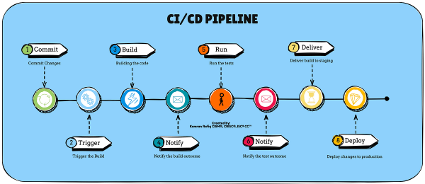
\includegraphics[width=1\linewidth]{figures/CI-CD.png}
    \caption{Standard CI/CD pipeline flow, illustrating the automated stages from code commit through build, test execution, notification, staging delivery, and production deployment.}
    \label{fig:cicd-pipeline}
\end{figure}

\textbf{Communication Archives} (Slack, Microsoft Teams, Google Chat, mailing lists) capture informal coordination events, though they present additional challenges for structured event extraction due to their unstructured nature.

The challenge for process mining lies not in the availability of data but in its integration: constructing a coherent event log from these heterogeneous sources requires resolving identifier mappings, temporal alignment, and semantic harmonization across tools with different data models~\cite{kochhar2019moving}. When raw event logs from these diverse sources are fed directly into discovery, conformance, and enhancement techniques, the resulting process models tend to exhibit spaghetti-like complexity that resists meaningful interpretation. As systematized by~\cite{Dixit2021}, applying preprocessing steps such as filtering, clustering, and transformation to the event log prior to mining yields structured and comprehensible models. Figure~\ref{fig:preprocessing-process-mining} contrasts these two settings: the traditional approach (a), where raw logs produce tangled models, and the expected approach (b), where preprocessing produces interpretable results. \cite{Dixit2021} classify these preprocessing techniques into two main families: transformation (filtering and time-based correction) and detection/visualization (pattern identification and anomaly detection).

\begin{figure}
    \centering
    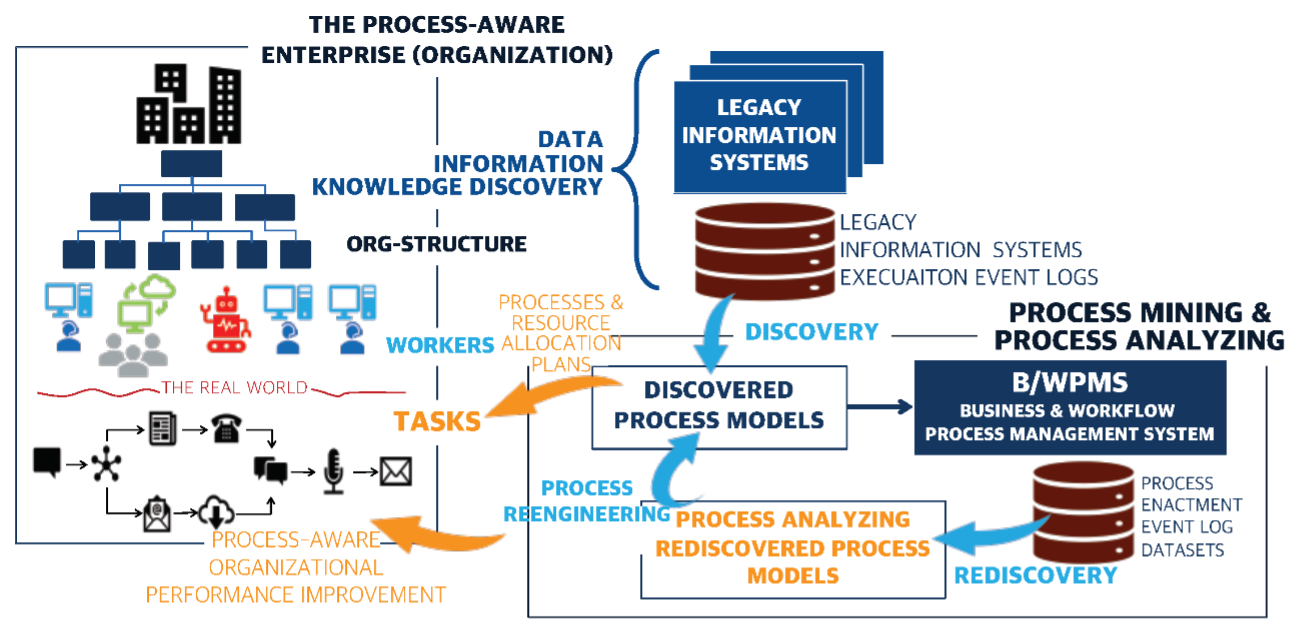
\includegraphics[width=1\linewidth]{figures/The Process-Awares.png}
    \caption{Traditional versus expected setting for applying process mining techniques. In the traditional approach (a), raw event logs are directly used, often resulting in complex, spaghetti-like process models. In the expected approach (b), preprocessing steps such as filtering, clustering, and transformation are applied to the event log before mining, yielding structured and interpretable process models. Adapted from \cite{Dixit2021}.}
    \label{fig:preprocessing-process-mining}
\end{figure}

This preprocessing concern is part of a broader organizational cycle. As depicted in Figure~\ref{fig:process-aware-enterprise}, a process-aware enterprise connects legacy information systems, whose execution event logs feed process mining and analysis techniques, to Business and Workflow Process Management Systems (B/WPMS), which operationalize the discovered models. The enactment of these models generates new event log datasets, enabling rediscovery and closing the continuous improvement loop through successive rounds of process reengineering. This cycle bridges the real world, where workers execute tasks across the tools described above, to the digital representation of processes through discovery, analysis, and reengineering stages~\cite{vanderAalst2009PAIS, vanderAalst2011PM}.

\begin{figure}
    \centering
    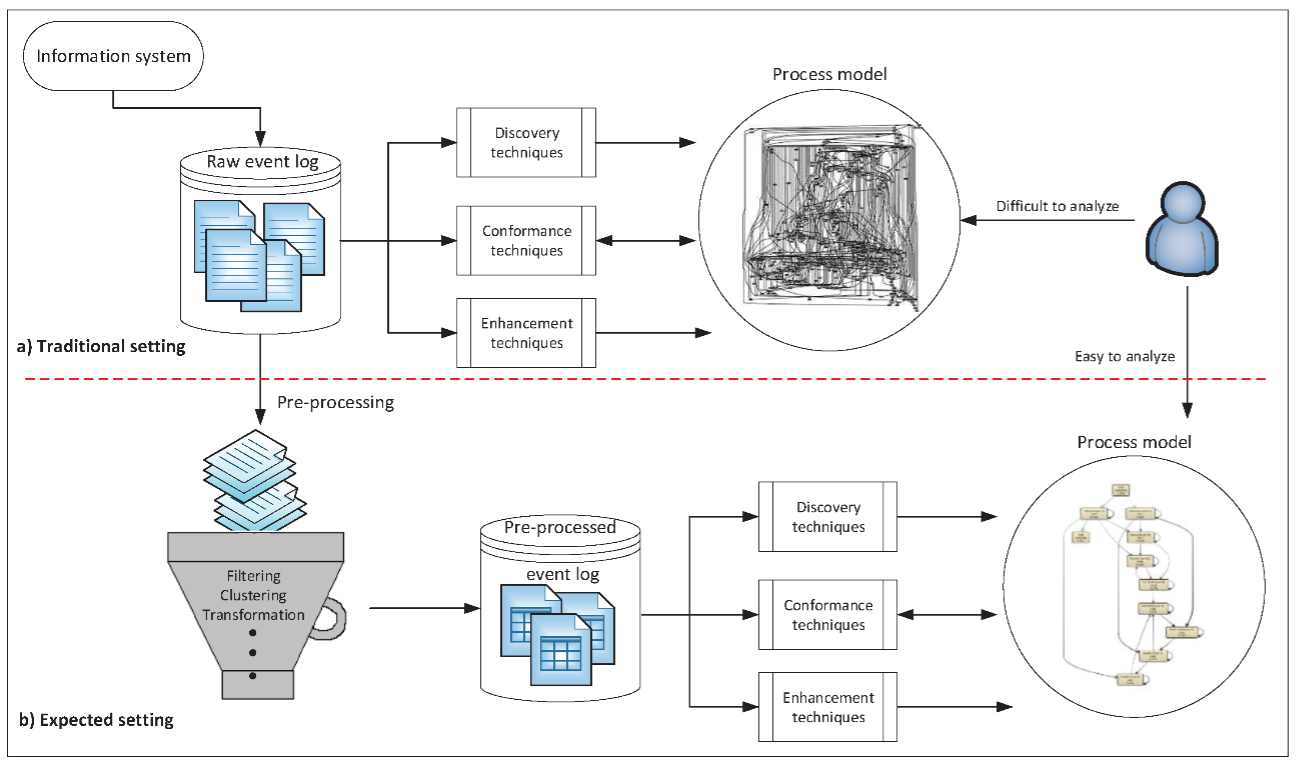
\includegraphics[width=1\linewidth]{figures/Process Analisys.png}
    \caption{The process-aware enterprise and the process mining cycle. Legacy information systems produce execution event logs that are used for process discovery. The discovered models feed Business and Workflow Process Management Systems (B/WPMS), whose enactment logs enable rediscovery and reengineering, closing the continuous improvement loop. Adapted from~\cite{vanderAalst2009PAIS}.}
    \label{fig:process-aware-enterprise}
\end{figure}

% --- 2.2.2 Repository Dataset Infrastructure and Collection Tooling ---
\subsection{Repository Dataset Infrastructure and Collection Tooling}
\label{sec:msr-dataset-infra}

The practical challenge of constructing a dataset of software repositories
for empirical studies has produced a range of specialised tools and curated
datasets that reduce the cost of candidate generation, filtering, and data
collection. Understanding their coverage and limitations is necessary for
designing selection protocols that are both valid and reproducible.

\paragraph{SEART GitHub Search.}
Dabic et al.~\cite{seart2021} built the SEART GitHub Search engine, a
web interface and API for querying GitHub repositories with filters not
available in the native GitHub search, including minimum commit counts,
issue and pull request availability, fork exclusion, and primary language
constraints. SEART is maintained by the Software Institute at
Università della Svizzera italiana and is widely used in MSR studies as a
reproducible candidate generation mechanism. Its query parameters map
directly onto the selection criteria defined in
Section~\ref{sec:selection-criteria}, making it the practical entry point
for the dataset construction protocol described in
Section~\ref{sec:selection-process}.

\paragraph{GH Archive.}
GH Archive~\cite{gharchive2023} records all public GitHub events since
2011 in newline-delimited JSON, compressed and partitioned by hour, and
makes the full archive queryable via Google BigQuery. It covers push
events, issue events, pull request events, and fork events, enabling
retrospective reconstruction of repository activity at arbitrary temporal
resolution. Because GH Archive captures events as they occur, its coverage
is complete for repositories that were public at the time of the event.
Its primary use in empirical SE studies is for large-scale trend analysis
and for identifying repositories that satisfy temporal activity criteria.

\paragraph{RepoReapers.}
Munaiah et al.~\cite{munaiah2017reporeapers} published a curated dataset
of approximately 1.8 million GitHub repositories classified along seven
engineering dimensions: commits, issues, pull requests, contributors,
branches, watchers, and forks. The classification enables the exclusion of
trivial, toy, or single-developer projects from empirical studies,
addressing the perils identified by Kalliamvakou et
al.~\cite{kochhar2019moving} regarding the non-representative nature of a
large proportion of public GitHub repositories. RepoReapers was
constructed in 2017 and requires verification against the current state of
repositories before use in contemporary studies.

\paragraph{SmartSHARK.}
Trautsch et al.~\cite{trautsch2020smartshark} published the SmartSHARK
dataset, which provides integrated Git, Jira, and CI data for Apache
Software Foundation projects. SmartSHARK was constructed for process
mining and software analytics studies and is notable as the only publicly
available dataset that pre-integrates all three data sources relevant to
PATHCAST event log construction. Its project-level coverage is narrower
than general-purpose GitHub datasets, but its data quality and
integration completeness make it suitable for controlled evaluations.

\paragraph{GrimoireLab.}
Dueñas et al.~\cite{dueenas2021grimoirelab} developed under the CHAOSS
initiative, is an open-source toolchain for the automated collection and
normalization of software development metrics from heterogeneous sources,
including Git, GitHub, Jira, Gerrit, and mailing lists. GrimoireLab
produces structured outputs compatible with process mining ingestion
pipelines and has been used as a data collection backbone in several
empirical SE studies. Its modular architecture allows independent
deployment of source-specific extractors, which is architecturally
analogous to the Stage~1 extraction adapters of the PATHCAST pipeline.

\paragraph{Public Jira Dataset.}
Montgomery et al.~\cite{montgomery2022jira} published a dataset covering
1,822 projects and 2.7 million issues with 32 million historical
state-change records, collected from 16 public Jira instances. The dataset
is anonymised at the user level while preserving uniqueness through UUID
masks, enabling contributor counting and resource-aware analysis without
exposing personal data. For projects that maintain a public Jira instance
alongside a GitHub repository, this dataset provides substantially richer
issue transition history than what is available through the GitHub Issues
timeline events API, which has known gaps for projects that migrated from
Jira to GitHub Issues.

\paragraph{Limitations of infrastructure-based collection.}
These tools and datasets collectively address the practical barriers to
large-scale repository mining but do not eliminate the fundamental
validity threats documented by Kalliamvakou et
al.~\cite{kochhar2019moving}: selection bias toward open-source,
English-language, GitHub-hosted projects; noise from bot-generated events;
and the incompleteness of observable development activity. The selection
criteria and exclusion filters defined in
Section~\ref{sec:selection-criteria} are designed to mitigate these
threats within the constraints imposed by data availability.


% --- 2.2.2 (old numbering) now renumbered ---
\subsection{The Bridge Between MSR and Process Mining}
\label{sec:msr-pm-bridge}

The intellectual bridge between MSR and process mining was established
incrementally over two decades. Cook and Wolf~\cite{cook1998} are recognized as the pioneers of applying process discovery to software, though their work predates the formalization of ``process mining'' as a discipline. Working at the University of Colorado, they demonstrated that state-machine models could be automatically discovered from event-based data recorded during software builds, establishing the feasibility of treating software development as a process amenable to formal analysis.

Rubin et al.~\cite{rubin2007} proposed an explicit framework---to the
best of our knowledge, among the earliest named frameworks for software
process mining---identifying five dimensions of analysis: process model
extraction, performance measurement, organizational mining, conformance
checking, and decision mining. Their framework mapped traditional process
mining capabilities to the software engineering domain, providing a
conceptual bridge that subsequent research could extend.

Poncin et al.~\cite{poncin2011process} formalized the intersection by
proposing a systematic methodology for mining software repositories with
process mining techniques. Their approach introduced the concept of
combining data from multiple repositories (version control, issue
trackers, mailing lists) into a unified event log, addressing the
multi-source integration challenge that distinguishes software process
mining from traditional BPM process mining. They demonstrated the
approach on open-source projects, revealing process patterns not visible
through artifact-level MSR analysis alone.

More recently, Caldeira and Cardoso~\cite{Caldeira2019AssessingSoftwareTeams} applied
process mining to assess software development processes in industrial
settings, demonstrating the practical applicability of the approach to
real-world development teams using modern tool chains (Jira, Git,
Jenkins). Their work highlighted both the analytical value of process
mining for software teams and the persistent challenges of event log
construction quality.

The evolution of this bridge is relevant because PATHCAST builds
upon it: the event log construction stage (Stage 1) operationalizes the
MSR-to-PM transformation, while subsequent stages extend the analytical
depth from descriptive discovery to probabilistic forecasting.


% --- 2.2.3 Event Log Construction from Software Repositories ---
\subsection{Event Log Construction from Software Repositories}
\label{sec:event-log-construction}

Constructing a process mining event log from raw software repository data
is the foundational challenge for any application of process mining to
SDLC~\cite{poncin2011process}. The transformation involves three
sub-tasks: event extraction, case correlation, and activity mapping.

\textbf{Event Extraction} involves retrieving timestamped records from
source systems. For issue trackers, this means extracting the changelog
of status transitions through REST APIs (e.g., Jira's \texttt{/issue/
\{key\}/changelog} endpoint). For Git repositories, it involves parsing
commit metadata. For CI/CD systems, it requires fetching pipeline run
records. Each source has its own API schema, authentication mechanism,
pagination strategy, and rate limiting constraints, requiring
source-specific extraction adapters.

\textbf{Case Correlation} maps extracted events to process instances
(cases). In traditional BPM, each event carries an explicit case
identifier because the process-aware information system generates the
log directly. In software development, events from different tools carry
different identifiers: an issue key in Jira, a commit hash in Git, a
PR number in GitHub, a build ID in Jenkins. Correlating these into a
unified case requires heuristic strategies: linking commits to issues
through message parsing (regex on commit messages), linking PRs to
issues through branch naming conventions or explicit references, and
linking builds to commits through CI trigger metadata.

The quality of case correlation directly impacts the quality of the
resulting process model. Incorrect correlations produce spurious
transitions in the process model; missed correlations produce incomplete
traces. This challenge motivates the formal treatment of correlation
quality metrics in the proposed method (Chapter~\ref{ch:method}).

\textbf{Activity Mapping} standardizes event labels into a common
taxonomy. Different tools use different terms for semantically equivalent
activities (e.g., ``In Development'' in Jira vs. ``Work in Progress'' in
Azure DevOps). Activity mapping defines a function
$\mu: \mathcal{A}_{\text{raw}} \rightarrow \mathcal{A}_{\text{standard}}$
that projects raw activity names onto a standardized vocabulary,
enabling cross-project and cross-tool comparability.

The entire construction process introduces threats to validity that
propagate through all downstream analyses. Events with incorrect
timestamps, misattributed cases, or wrong activity labels produce
process models that reflect construction artifacts rather than actual
process behavior. This observation motivates the quality metrics and
validation protocols defined in the methodology
(Chapter~\ref{ch:methodology}).


% --- 2.2.4 Data Quality Challenges ---
\subsection{Data Quality Challenges and Threats to Validity}
\label{sec:msr-quality}

The MSR literature has documented a range of data quality challenges that
affect any empirical study based on software repository
data~\cite{kochhar2019moving}.

\textbf{Perils of Mining GitHub.} Kalliamvakou et
al.~\cite{kochhar2019moving} identified 13 perils of mining GitHub
repositories, including: repositories that are not development projects
(forks, mirrors, data dumps); projects with no activity or minimal
collaboration; pull requests used for purposes other than code review;
and the bias toward English-speaking, open-source, GitHub-hosted projects.
These perils directly affect the construction of event logs because they
can introduce cases that do not represent genuine software development
processes.

\textbf{Timestamp Quality.} Software events are recorded with varying
temporal precision. Issue tracker transitions are timestamped at second
granularity (or coarser); Git commits carry author timestamps that may
not reflect the actual commit time (squashed commits, rebased branches,
timezone inconsistencies). CI/CD events are typically timestamped by the
server, providing reliable temporal data. When constructing event logs,
temporal ordering within a case is based on these timestamps, and
ordering errors produce incorrect transition sequences.

\textbf{Bot and Automation Activity.} Automated tools (bots, CI triggers,
auto-assignment rules) generate events that interleave with human
activity. These automated events may inflate activity frequencies and
distort process models. Filtering bot activity requires heuristics based
on actor identification (e.g., usernames matching bot patterns) and
event timing (e.g., transitions occurring within milliseconds of a
trigger event).

\textbf{Process Variability.} Unlike manufacturing or healthcare
processes, software development processes exhibit high variability across
teams, projects, and time periods. The same organization may have
different workflow configurations for different project types (bug fixes
vs. feature development), teams (frontend vs. backend), or maturity
levels (startup vs. established product). This variability means that a
single process model may not adequately represent all cases in the log,
requiring either case-level filtering or multi-model
approaches~\cite{dambros2012evaluating}.

\textbf{Incompleteness.} Not all process activities leave digital traces.
Informal conversations, whiteboard discussions, and ad-hoc decisions
occur outside tracked systems. The resulting event log captures only the
observable portion of the process, potentially missing transitions that
occur through non-instrumented channels. This systematic incompleteness
means that discovered process models represent a lower bound on the
complexity of actual development processes.


% --- 2.2.5 Software Process Mining: State of the Art ---
\subsection{Software Process Mining: State of the Art}
\label{sec:software-pm-sota}

The application of process mining to software development has grown
steadily since Cook and Wolf's seminal work. Key themes in the literature
include:

\textbf{Process Discovery from Issue Trackers.} Multiple studies have
applied process discovery algorithms to issue tracker data, extracting
workflow models from Jira, Bugzilla, and GitHub Issues~\cite{Caldeira2019AssessingSoftwareTeams,lemos2011using}. The resulting models
reveal the actual development process, including rework loops, parallel
activities, and exception paths that are absent from prescribed workflow
definitions. Lemos et al.~\cite{lemos2011using} demonstrated the use of
process mining for software development process management, showing how
discovered models could identify bottlenecks and compliance issues.

\textbf{Multi-Repository Mining.} Integrating data from multiple
repositories into a unified process view remains an active research
challenge. Poncin et al.~\cite{poncin2011process} proposed combining
data from VCS, issue trackers, and mailing lists. Subsequent work has
extended this to include code review systems, CI/CD pipelines, and
project management tools, though the case correlation challenge persists
as the primary barrier to scalable multi-source mining.

\textbf{Performance and Bottleneck Analysis.} Process enhancement
applied to software development has revealed patterns such as prolonged
code review cycles, testing bottlenecks due to shared environments, and
deployment delays caused by release window constraints. These findings
inform process improvement initiatives and motivate the quantitative
forecasting approach proposed in this thesis.

\textbf{Conformance Checking for Process Compliance.} Organizations
with prescribed development processes (e.g., ISO 12207, CMMI-based
workflows) can use conformance checking to verify adherence to defined
procedures. Deviations identified through conformance analysis serve both
compliance purposes and as diagnostic indicators of process maturity.

The common thread across this literature is that the analytical depth
remains concentrated at the descriptive and diagnostic levels (discovery,
conformance, bottleneck detection). The progression toward predictive and
forecasting capabilities, which requires integrating process mining with
stochastic modeling and machine learning, remains nascent. 

This observation motivates adopting a reconstruction-focused perspective on repository traces, which we discuss next as an evidential prerequisite for process-aware forecasting and which, in turn, underlies the gap analysis presented in Section~\ref{sec:related-work}.


% --- 2.2.6 Software Process Archaeology ---
\subsection{Software Process Archaeology}

The term \emph{software archaeology} refers to the extraction of organizational and process knowledge from legacy software artifacts, particularly version control histories, issue tracking records, and build or deployment traces \cite{Zimmermann2005MiningVersionHistories}. The metaphor is useful because it emphasizes that software repositories do not provide a direct and complete representation of the development process. Instead, they preserve partial traces from which aspects of past process execution can be reconstructed.

In the context of this thesis, software process archaeology is not introduced as an independent research objective, but as an evidential foundation for probabilistic forecasting. Its role is to support the reconstruction of historically grounded event logs from heterogeneous repositories so that downstream forecasting models can rely on explicit process structure rather than on aggregated black-box metrics alone.

This distinction is important. The primary goal of the thesis is not to interpret the past for its own sake, but to improve the prediction of future process behavior. Accordingly, archaeological reconstruction is relevant here only insofar as it enables the PATHCAST pipeline to identify comparable process states, estimate transition behavior, and generate probabilistic forecasts at the case level. In operational terms, the pipeline follows the sequence:
\[
\text{event log} \rightarrow \text{Markov chains} \rightarrow \text{Monte Carlo simulation} \rightarrow \text{machine learning}.
\]
The unit of analysis is the individual case, such as an issue or work item, and the primary outputs are probability distributions over completion time and outcome.

From this perspective, software process archaeology functions as an upstream reconstruction layer. It establishes the empirical conditions required for process-aware forecasting by making past execution traces suitable for process mining and stochastic modeling. If this reconstruction is weak, incomplete, or inconsistent, the resulting forecasts will inherit these limitations regardless of the sophistication of the downstream analytical techniques.

Three principles from the archaeological metaphor are especially relevant to this thesis.

\textbf{Stratigraphic analysis.} Events recorded in different time periods may reflect distinct process configurations, team structures, toolchains, and working agreements. Temporal stratification is therefore necessary to identify process evolution and to select analysis windows that are sufficiently stable for estimating stochastic dynamics.

\textbf{Contextual interpretation.} A commit, review event, issue transition, or build signal must be interpreted in relation to the project context in which it occurred. Naming conventions, workflow customizations, and tool-specific semantics affect how raw traces should be mapped into process activities and states. Without this contextualization, the event log may mix heterogeneous meanings under the same label, weakening both model validity and forecast quality.

\textbf{Taphonomic bias.} Not all development activities are equally preserved in digital repositories. Activities executed within tracked systems leave explicit traces, whereas informal coordination, undocumented work, and off-system decisions often leave none. Consequently, the observable event log is a biased representation of the actual process. In this thesis, such bias is treated as a boundary condition for forecasting, since predictions can only be as complete as the process evidence on which they are based.

Therefore, software process archaeology should be understood here as a methodological prerequisite for PATHCAST rather than as a parallel contribution. It provides the empirical grounding that allows process mining to recover executable structure, Markov models to estimate transition dynamics, Monte Carlo simulation to quantify uncertainty, and machine learning to incorporate process-derived predictive signals. The scientific contribution of the thesis remains centered on forecasting, while archaeological reconstruction serves as the necessary bridge between raw repository traces and forecast-ready process representations.


% =============================================================================
% 2.3 STOCHASTIC PROCESS MODELING WITH MARKOV CHAINS
% =============================================================================
\section{Stochastic Process Modeling with Markov Chains}
\label{sec:markov}

Software delivery systems, whether expressed as SDLC stages, CI/CD
pipelines, or service workflows, evolve through discrete states (e.g.,
Backlog, In Progress, Review, Testing, Done). These systems are
inherently stochastic: queueing effects, rework, blocking, variable
service times, and human decision-making introduce uncertainty at every
transition. Discrete-time Markov chains (DTMCs) provide a mathematically
rigorous formalism to model such systems as state-transition dynamics,
enabling quantitative prediction of future paths, time-to-completion,
and outcome probabilities~\cite{Spedicato2017, Haggstrom2002}.

Unlike approaches based on aggregated metrics, modeling through Markov chains makes it possible to capture the transition structure of the process, thereby capturing path dependencies and rework effects that characterize real-world software development processes.

This section presents the mathematical foundations of DTMCs with emphasis
on the concepts directly employed by the PATHCAST method: the
Markov property, transition matrices, absorbing chains, the fundamental
matrix, sojourn time distributions, and parameter estimation from event
logs.


% --- 2.3.1 Discrete-Time Markov Chains ---
\subsection{Discrete-Time Markov Chains}
\label{sec:dtmc}

\begin{definition}[Discrete-Time Markov Chain]
\label{def:dtmc}
Let $S = \{1, \ldots, m\}$ be a finite set of states. A stochastic
process $\{X_t\}_{t \in \mathbb{N}}$ taking values in $S$ is a
discrete-time Markov chain (DTMC) if for all $t \geq 0$ and all states
$i_0, \ldots, i_t, j \in S$:
\begin{equation}
\label{eq:markov-property}
P(X_{t+1} = j \mid X_t = i_t, X_{t-1} = i_{t-1}, \ldots, X_0 = i_0)
= P(X_{t+1} = j \mid X_t = i_t)
\end{equation}
This is the \emph{Markov property} (memorylessness): the probability of
transitioning to a future state depends only on the current state, not
on the history of previously visited states.
\end{definition}

When the transition probabilities do not depend on $t$, the chain is
\emph{time-homogeneous}, and a single transition matrix suffices to
describe all dynamics.

\begin{definition}[Transition Matrix]
\label{def:transition-matrix}
The transition probabilities $p_{ij} = P(X_{t+1} = j \mid X_t = i)$
form a matrix $P = [p_{ij}]_{i,j=1}^{m}$ satisfying the row-stochastic
constraints:
\begin{equation}
\label{eq:row-stochastic}
p_{ij} \geq 0 \quad \forall\, i,j \in S, \qquad
\sum_{j=1}^{m} p_{ij} = 1 \quad \forall\, i \in S
\end{equation}
\end{definition}

\textbf{Chapman-Kolmogorov Equations.} Multi-step transition
probabilities satisfy the Chapman-Kolmogorov equations, which state that
the $n$-step transition probability from state $i$ to state $j$ is
obtained by summing over all intermediate states at any intermediate
step:
\begin{equation}
\label{eq:chapman-kolmogorov}
p_{ij}^{(n)} = \sum_{k \in S} p_{ik}^{(r)} \cdot p_{kj}^{(n-r)}
\quad \text{for any } 0 \leq r \leq n
\end{equation}
In matrix form, this simplifies to $P^{(n)} = P^n$: the $n$-step
transition matrix is the $n$-th power of the one-step matrix $P$. This
property is computationally valuable because it enables the derivation of
multi-step behavior from a single estimated matrix.

The state distribution at time $t$ is a row vector $\pi^{(t)}$ satisfying
$\pi^{(t)} = \pi^{(0)} P^t$, where $\pi^{(0)}$ is the initial state
distribution. In the SDLC context, $\pi^{(0)}$ represents the initial
distribution of work items across workflow states, and $\pi^{(t)}$
predicts the distribution after $t$ transitions.

\begin{definition}[Stationary Distribution]
\label{def:stationary}
A probability row vector $\pi$ is \emph{stationary} (or \emph{invariant})
if $\pi = \pi P$. For a finite, irreducible, and aperiodic DTMC, a unique
stationary distribution exists, and $\lim_{t \to \infty} \pi^{(0)} P^t =
\pi$ for any initial distribution $\pi^{(0)}$.
\end{definition}

In the SDLC context, the stationary distribution $\pi_i$ approximates the
long-run fraction of work items in state $i$, providing an interpretable
baseline for WIP (Work-in-Progress) decomposition and capacity assessment.

\textbf{Classification of States.} States in a DTMC are classified according
to communication properties:

A state $j$ is \emph{accessible} from state $i$ (written $i \rightarrow j$)
if there exists $n \geq 0$ such that $p_{ij}^{(n)} > 0$. Two states
communicate ($i \leftrightarrow j$) if each is accessible from the other.
Communication is an equivalence relation, partitioning the state space
into \emph{communicating classes}.

A state is \emph{recurrent} if, starting from that state, the chain returns
to it with probability 1; otherwise it is \emph{transient}. A chain is
\emph{irreducible} if all states belong to a single communicating class.
A chain is \emph{absorbing} if it contains absorbing states (states from
which no exit is possible), which is the case relevant for SDLC modeling
where ``Done'' and ``Cancelled'' are terminal states.


% --- 2.3.2 Absorbing Chains and the Fundamental Matrix ---
\subsection{Absorbing Chains and the Fundamental Matrix}
\label{sec:absorbing-chains}

Software development processes have natural terminal states (Done,
Cancelled, Deployed). Once a work item reaches a terminal state, it
remains there indefinitely. Modeling these processes as absorbing Markov
chains enables the computation of expected completion times and outcome
probabilities through closed-form expressions.

\begin{definition}[Absorbing State and Absorbing Chain]
\label{def:absorbing}
A state $a$ is \emph{absorbing} if $p_{aa} = 1$ (equivalently, $p_{aj} = 0$
for all $j \neq a$). A DTMC is an \emph{absorbing chain} if (i) it has at
least one absorbing state, and (ii) every non-absorbing (transient) state
can reach at least one absorbing state in a finite number of steps.
\end{definition}

For an absorbing chain with $t$ transient states and $r$ absorbing states
($m = t + r$), the transition matrix can be reordered into canonical form:

\begin{equation}
\label{eq:absorbing-form}
P = \begin{pmatrix} Q & R \\ \mathbf{0} & I_r \end{pmatrix}
\end{equation}

where $Q \in [0,1]^{t \times t}$ contains transition probabilities among
transient states, $R \in [0,1]^{t \times r}$ contains transition
probabilities from transient to absorbing states, $\mathbf{0}$ is the
$r \times t$ zero matrix (absorbing states cannot reach transient states),
and $I_r$ is the $r \times r$ identity matrix (absorbing states remain
absorbing).

\begin{definition}[Fundamental Matrix]
\label{def:fundamental-matrix}
The fundamental matrix of an absorbing chain is:
\begin{equation}
\label{eq:fundamental}
N = (I_t - Q)^{-1} = \sum_{k=0}^{\infty} Q^k
\end{equation}
where $I_t$ is the $t \times t$ identity matrix. The entry $n_{ij}$
gives the \emph{expected number of times} the chain visits transient
state $j$ given that it starts in transient state $i$, before being
absorbed.
\end{definition}

The fundamental matrix exists and is unique because, in an absorbing chain,
the spectral radius of $Q$ is strictly less than 1, guaranteeing the
convergence of the geometric series $\sum Q^k$ and the invertibility of
$(I_t - Q)$.

\begin{theorem}[Properties of Absorbing Chains]
\label{thm:absorption}
For an absorbing chain with fundamental matrix $N = (I - Q)^{-1}$,
the following properties hold:

\emph{(i) Expected number of steps to absorption.} The expected number of
transitions before being absorbed, starting from transient state $i$, is:
\begin{equation}
\label{eq:expected-steps}
E[T_i] = (N \cdot \mathbf{1})_i = \sum_{j=1}^{t} n_{ij}
\end{equation}
where $\mathbf{1}$ is the column vector of ones.

\emph{(ii) Variance of steps to absorption.} The variance of the number
of transitions before absorption, starting from state $i$, is:
\begin{equation}
\label{eq:variance-steps}
\text{Var}(T_i) = \left( N(2N_{\text{dg}} - I) \cdot \mathbf{1} \right)_i
- E[T_i]^2
\end{equation}
where $N_{\text{dg}}$ is the diagonal matrix formed from the diagonal
entries of $N$.

\emph{(iii) Absorption probabilities.} The probability of being absorbed
in absorbing state $a_j$, starting from transient state $i$, is:
\begin{equation}
\label{eq:absorption-prob}
B = N \cdot R
\end{equation}
where $B_{ij}$ gives the probability that a chain starting in transient
state $i$ is eventually absorbed in absorbing state $j$.
\end{theorem}

\begin{proof}
Property (i): The expected number of visits to state $j$ starting from
$i$ is $n_{ij} = \delta_{ij} + \sum_k p_{ik} n_{kj}$, which in matrix
form yields $N = I + QN$, hence $N = (I - Q)^{-1}$. Summing row $i$
gives the total expected visits across all transient states before
absorption.

Property (ii): Let $T_i$ be the absorption time from state $i$. By the
law of total expectation and variance, conditioning on the first step
and using the matrix $N$, the variance follows from
$E[T_i^2] = (N(2N_{\text{dg}} - I) \cdot \mathbf{1})_i$, from which
$\text{Var}(T_i) = E[T_i^2] - (E[T_i])^2$.

Property (iii): The probability of eventually reaching absorbing state
$a_j$ from transient state $i$ is $\sum_{k} n_{ik} r_{kj}$, where
$n_{ik}$ counts expected visits to $k$ and $r_{kj}$ is the one-step
probability from $k$ to $a_j$. In matrix form, $B = NR$.
\end{proof}

In the SDLC context, property (i) provides the expected number of
transitions before a work item reaches a terminal state, property (ii)
quantifies the uncertainty in this estimate, and property (iii) predicts
the probability of different outcomes (e.g., probability of completion
vs. cancellation). These closed-form results provide analytical baselines
against which Monte Carlo simulation results can be validated.


% --- 2.3.3 Sojourn Time Distributions ---
\subsection{Sojourn Time Distributions}
\label{sec:sojourn-time}

The DTMC framework models transitions between states but does not
inherently capture the time spent in each state. In software development,
the sojourn time, the duration a work item spends in a given state before
transitioning, varies substantially due to task complexity, resource
availability, and external dependencies. Extending the Markov model with
sojourn time distributions transforms it from a purely structural model
(capturing transition probabilities) into a temporal model (capturing both
transition probabilities and timing).

\begin{definition}[Sojourn Time]
\label{def:sojourn-time}
Let $\sigma_c = \langle e_1, \ldots, e_n \rangle$ be a trace and let
$e_k, e_{k+1}$ be consecutive events with $\alpha(e_k) \neq
\alpha(e_{k+1})$ (i.e., a state transition occurs). The sojourn time in
state $s = \alpha(e_k)$ for this visit is
$\Delta t_s = \tau(e_{k+1}) - \tau(e_k)$.
\end{definition}

The collection of all observed sojourn times for state $s$ across all
traces in the event log forms an empirical distribution:
$\hat{F}_s = \{\Delta t_s^{(1)}, \Delta t_s^{(2)}, \ldots, \Delta
t_s^{(n_s)}\}$, where $n_s$ is the total number of visits to state $s$.

\textbf{Distributional Fitting.} Empirical sojourn time distributions in
software development are typically right-skewed and heavy-tailed: most
work items progress through a state relatively quickly, but a fraction
experiences extended delays due to blocking, rework, or resource
contention. Common parametric families used to model sojourn times
include:

\begin{itemize}
    \item \textbf{Lognormal}: $\Delta t \sim \text{LogNormal}(\mu,
    \sigma^2)$, appropriate when the logarithm of sojourn times is
    approximately normal. This is common for development and review states.
    \item \textbf{Gamma}: $\Delta t \sim \text{Gamma}(\alpha, \beta)$,
    providing flexible shape for both symmetric and skewed distributions.
    \item \textbf{Exponential}: $\Delta t \sim \text{Exp}(\lambda)$, the
    memoryless distribution, appropriate when the time to the next
    transition does not depend on how long the item has been in the
    current state. This corresponds to a continuous-time Markov chain
    (CTMC) assumption.
    \item \textbf{Weibull}: $\Delta t \sim \text{Weibull}(\lambda, k)$,
    generalizing the exponential with a shape parameter that captures
    increasing ($k > 1$) or decreasing ($k < 1$) hazard rates.
\end{itemize}

In PATHCAST, a pragmatic approach is adopted: rather than committing
to a specific parametric family, the empirical distribution $\hat{F}_s$
is used directly for sampling in Monte Carlo simulations. This
non-parametric approach avoids model misspecification (choosing the wrong
distributional family) at the cost of requiring sufficient sample sizes
per state. When sample sizes are small, kernel density estimation (KDE)
or parametric fitting with model selection (e.g., AIC/BIC comparison)
can be employed as alternatives.

\textbf{Mean Sojourn Time.} The mean sojourn time for state $s$ is:
\begin{equation}
\label{eq:mean-sojourn}
\bar{T}_s = \frac{1}{n_s} \sum_{k=1}^{n_s} \Delta t_s^{(k)}
\end{equation}
When combined with the expected number of visits from the fundamental
matrix ($n_{is}$), the expected total time spent in state $s$ starting
from state $i$ is $n_{is} \cdot \bar{T}_s$, and the expected total
lead time from state $i$ to absorption is:
\begin{equation}
\label{eq:expected-lead-time}
E[\text{LT}_i] = \sum_{s \in S_t} n_{is} \cdot \bar{T}_s
\end{equation}
where $S_t$ is the set of transient states. This formula provides a
closed-form estimate of expected lead time that serves as a baseline
for the Monte Carlo simulation.


% --- 2.3.4 Semi-Markov Processes ---
\subsection{Semi-Markov Processes and the Markov Renewal Framework}
\label{sec:semi-markov}

The augmentation of DTMCs with empirical sojourn time distributions, as
described above, produces a model that is formally related to the
Semi-Markov Process (SMP) framework. Understanding this connection
clarifies the theoretical positioning of the PATHCAST simulation
model.

\begin{definition}[Semi-Markov Process]
\label{def:semi-markov}
A Semi-Markov Process is a stochastic process $\{Z(t)\}_{t \geq 0}$
defined by:
\begin{enumerate}
    \item A DTMC $\{X_n\}_{n \in \mathbb{N}}$ with transition matrix $P$
    governing the sequence of states visited (the \emph{embedded chain});
    \item A set of sojourn time distributions
    $\{H_{ij}(\cdot)\}_{i,j \in S}$ where $H_{ij}(t)$ is the probability
    that the sojourn time in state $i$ is at most $t$, given that the
    next state is $j$.
\end{enumerate}
The process remains in state $X_n$ for a random time drawn from
$H_{X_n, X_{n+1}}$ before transitioning to $X_{n+1}$.
\end{definition}

The Semi-Markov Process generalizes both the DTMC (where sojourn times
are deterministic and equal to one time unit) and the Continuous-Time
Markov Chain (CTMC, where sojourn times are exponentially distributed
with state-dependent rates). The SMP framework is more expressive than
either because it permits arbitrary sojourn time distributions,
accommodating the right-skewed, heavy-tailed distributions empirically
observed in software development processes.

When sojourn time distributions do not depend on the next state
(i.e., $H_{ij}(t) = H_i(t)$ for all $j$), the SMP simplifies to a
\emph{Markov Renewal Process} with state-dependent holding times. This
is the model implicitly adopted by PATHCAST: the sojourn time in
state $s$ is drawn from $\hat{F}_s$ regardless of which state is visited
next. This simplification is justified when the primary determinant of
sojourn time is the state itself (e.g., the ``Code Review'' state has
a characteristic duration distribution regardless of whether the next
transition leads to ``Testing'' or back to ``In Progress'').

\textbf{Quasi-Stationary Distribution.} For absorbing Semi-Markov
processes, the quasi-stationary distribution characterizes the long-run
proportion of time spent in each transient state, conditional on not
yet being absorbed. The quasi-stationary distribution $\pi^q$ satisfies:
\begin{equation}
\label{eq:quasi-stationary}
\pi^q_i = \frac{\sum_j n_{ji} \cdot \bar{T}_i}
{\sum_{k \in S_t} \sum_j n_{jk} \cdot \bar{T}_k}
\end{equation}
where $n_{ji}$ are entries of the fundamental matrix and $\bar{T}_i$
is the mean sojourn time in state $i$. This distribution provides
insight into where work items spend most of their time before completion,
informing bottleneck analysis and capacity planning.

The formal connection to Semi-Markov theory provides theoretical
grounding for the PATHCAST simulation model: the simulation in
Algorithm~\ref{alg:mc-simulation} is, in effect, a Monte Carlo
estimator for the properties of an absorbing Semi-Markov process
parameterized by the discovered process model.


% --- 2.3.4 Estimating Transition Probabilities from Event Logs ---
\subsection{Estimating Transition Probabilities from Event Logs}
\label{sec:markov-estimation}

Given an event log $\mathcal{L}$, the transition probabilities of the
Markov chain must be estimated from observed state transitions. The
standard approach is Maximum Likelihood Estimation (MLE).

Let $c_{ij}$ denote the number of observed transitions from state $i$ to
state $j$ across all traces in $\mathcal{L}$. The MLE estimator for the
transition probability is:
\begin{equation}
\label{eq:mle-transition}
\hat{p}_{ij} = \frac{c_{ij}}{\sum_{k \in S} c_{ik}}
= \frac{c_{ij}}{c_{i \cdot}}
\end{equation}
where $c_{i \cdot} = \sum_k c_{ik}$ is the total number of transitions
out of state $i$.

The MLE estimator is the maximum likelihood solution for the multinomial
distribution of transitions from each state: given $c_{i\cdot}$
transitions from state $i$, the likelihood of the observed transition
counts is:
\begin{equation}
\label{eq:mle-full}
L(P_i \mid \text{data}) = \frac{c_{i\cdot}!}{\prod_j c_{ij}!}
\prod_{j \in S} p_{ij}^{c_{ij}}
\end{equation}
Maximizing the log-likelihood subject to $\sum_j p_{ij} = 1$ yields
Equation~\ref{eq:mle-transition}.

\textbf{The Zero-Count Problem.} When a transition $i \rightarrow j$ is
never observed in the log ($c_{ij} = 0$), the MLE assigns
$\hat{p}_{ij} = 0$, making the transition structurally impossible in
the model. This can be problematic when the absence of a transition
reflects insufficient data rather than genuine impossibility. Laplace
(additive) smoothing addresses this by adding a pseudo-count $\alpha > 0$:
\begin{equation}
\label{eq:laplace-smoothing}
\hat{p}_{ij}^{(\alpha)} = \frac{c_{ij} + \alpha}
{c_{i\cdot} + \alpha \cdot |S|}
\end{equation}
With $\alpha = 1$ (uniform prior), this corresponds to the posterior mean
under a symmetric Dirichlet prior $\text{Dir}(\mathbf{1})$.

In practice, the choice of $\alpha$ involves a trade-off: larger values
regularize the estimates toward uniformity (useful with sparse data),
while smaller values stay closer to the observed frequencies (useful with
abundant data). For software development logs with hundreds or thousands
of cases, MLE without smoothing is typically sufficient for states with
adequate coverage. Smoothing is reserved for transitions involving rare
states or states with fewer than 30 observed transitions, following the
standard statistical guideline for minimum sample size.

\textbf{Confidence in Estimates.} The uncertainty in estimated transition
probabilities can be quantified through the posterior distribution under
a Dirichlet-Multinomial model. Given counts $\mathbf{c}_i = (c_{i1},
\ldots, c_{im})$ and a Dirichlet prior $\text{Dir}(\boldsymbol{\alpha})$,
the posterior is:
\begin{equation}
\label{eq:posterior-transition}
P_i \mid \mathbf{c}_i \sim
\text{Dir}(c_{i1} + \alpha_1, \ldots, c_{im} + \alpha_m)
\end{equation}
The width of the posterior credible intervals decreases with
$c_{i\cdot}$, providing a natural measure of estimation reliability.
This Bayesian perspective is relevant for PATHCAST because it
enables the propagation of estimation uncertainty through the Monte Carlo
simulation.


% --- 2.3.5 Markov Models for SDLC State Transitions ---
\subsection{Markov Models for SDLC State Transitions}
\label{sec:markov-sdlc}

Applying DTMCs to SDLC processes requires defining a state space that
captures the workflow stages relevant for analysis. A typical SDLC
state space is:
\begin{equation}
\label{eq:sdlc-states}
S_{\text{SDLC}} = \{\underbrace{\text{Backlog}, \text{InProgress},
\text{Review}, \text{Testing}}_{\text{transient}},
\underbrace{\text{Done}, \text{Cancelled}}_{\text{absorbing}}\}
\end{equation}

This state space induces an absorbing Markov chain where ``Done'' and
``Cancelled'' are absorbing states and all other states are transient.
The transition matrix estimated from the event log captures the
probabilities of moving between states, including rework loops (e.g.,
Testing $\rightarrow$ InProgress with probability reflecting the
rework rate).

\textbf{Numerical Example.} Consider a project with 500 observed issues
and the following estimated transition matrix:

\begin{equation}
\label{eq:sdlc-example}
P = \bordermatrix{
  & \text{BL} & \text{IP} & \text{RV} & \text{TS} & \text{DN} & \text{CA} \cr
\text{BL} & 0 & 0.85 & 0 & 0 & 0 & 0.15 \cr
\text{IP} & 0 & 0 & 0.80 & 0.10 & 0 & 0.10 \cr
\text{RV} & 0 & 0.20 & 0 & 0.75 & 0.05 & 0 \cr
\text{TS} & 0 & 0.15 & 0 & 0 & 0.80 & 0.05 \cr
\text{DN} & 0 & 0 & 0 & 0 & 1 & 0 \cr
\text{CA} & 0 & 0 & 0 & 0 & 0 & 1 \cr
}
\end{equation}

From this matrix, the transient block is:
$Q = \begin{pmatrix} 0 & 0.85 & 0 & 0 \\ 0 & 0 & 0.80 & 0.10 \\
0 & 0.20 & 0 & 0.75 \\ 0 & 0.15 & 0 & 0 \end{pmatrix}$

Computing $N = (I - Q)^{-1}$ yields the expected number of visits per
state, and $N \cdot \mathbf{1}$ gives the expected number of transitions
before absorption. The matrix $B = NR$ gives the probability of ending
in Done vs. Cancelled from each starting state. For instance, starting
from Backlog, the chain might predict an 82\% probability of reaching
Done and an 18\% probability of cancellation, with an expected 5.3
transitions before absorption. These analytical results can then be
validated against Monte Carlo simulation output.


% --- 2.3.6 Limitations of the Markov Assumption ---
\subsection{Limitations of the Markov Assumption in Software Processes}
\label{sec:markov-limitations}

The first-order Markov assumption (memorylessness) states that the
probability of transitioning to the next state depends only on the
current state, not on how the process arrived at that state. This
assumption is a simplification that does not hold universally for
software development processes. Several limitations warrant discussion.

\textbf{History-Dependent Transitions.} A work item that reaches the
Testing state after being reworked from Review may have a different
probability of passing than an item reaching Testing for the first time.
The number of prior rework iterations, the severity of the defect, and
the experience of the assigned developer all create history dependencies
that the Markov assumption ignores.

\textbf{Time-Varying Transition Probabilities.} Transition probabilities
may change over time due to team learning, process improvements, or
external factors (e.g., a code freeze before a major release). The
assumption of time-homogeneous transitions may not hold across long
observation windows.

\textbf{State Aggregation.} The Markov property is sensitive to the
granularity of the state space. A process that is non-Markovian at a
coarse level of state aggregation may become approximately Markovian
at a finer level (e.g., distinguishing ``InProgress-FirstTime'' from
``InProgress-Rework''). This motivates state space refinement strategies.

\textbf{Mitigation Strategies.} Several approaches can mitigate these
limitations while preserving the computational tractability of the
Markov framework: (1) state space expansion to encode relevant history
(adding rework counters to states), (2) higher-order Markov models
($k$-th order chains where the state includes the last $k$ transitions),
(3) sliding window estimation to capture temporal variation, and
(4) combining the Markov model with a machine learning classifier that
captures non-Markovian features. The PATHCAST method adopts
strategy (4): the Markov chain captures the structural dynamics of the
process, and the ML component captures the residual variation not
explained by the Markov model.

\section{Flow Metrics and Probabilistic Forecasting in Software Engineering}
\label{sec:flow-metrics}

The Kanban method introduced a metrics-driven approach to software
delivery management grounded in queueing
theory~\cite{anderson2010kanban}. Four fundamental flow metrics form the
operational backbone of this approach: work in progress (WIP), cycle
time, throughput, and work item age~\cite{vacanti2015}. These metrics
are interconnected through Little's Law~\cite{little1961proof}, which
establishes that under steady-state conditions, the average number of
items in a system equals the product of the average arrival rate and the
average time each item spends in the system:

\begin{equation}
\label{eq:littles-law}
L = \lambda W
\end{equation}

\noindent where $L$ is the average WIP, $\lambda$ is the average
throughput, and $W$ is the average cycle time. This relationship holds
for any stable system regardless of the arrival distribution, service
distribution, or number of servers~\cite{little1961proof}, making it
applicable to software development processes provided the system
operates under approximately stationary conditions.

The practical implication for software teams is that cycle time
reduction can be achieved either by increasing throughput (requiring
capacity investment) or by limiting WIP (requiring only policy
changes)~\cite{anderson2010kanban, vacanti2015}. This insight
underpins the WIP limit practice in Kanban, which constrains the
number of concurrent items per workflow stage to stabilize the system
and improve predictability.

However, the direct application of Little's Law assumes thin-tailed
distributions and stable averages, conditions rarely met in
practice~\cite{savage2009flaw}. Software development lead times
exhibit heavy-tailed distributions where the mean is an unreliable
estimator and the variance may be
undefined~\cite{flyvbjerg2022empirical}. Savage~\cite{savage2009flaw}
formalized this limitation as the ``Flaw of Averages'': plans based on
average assumptions are wrong on average, because Jensen's inequality
implies that the average of a nonlinear function differs from the
function evaluated at the average input.

This limitation motivates the transition from deterministic forecasting
(single-point estimates derived from averages) to probabilistic
forecasting based on Monte Carlo
simulation~\cite{magennis2011forecasting, vacanti2020when}. Rather
than predicting a single delivery date, probabilistic forecasting
produces a distribution of possible outcomes, expressing forecasts as
confidence intervals (e.g., ``85\% probability of completing 20 items
by Sprint~12''). Magennis~\cite{magennis2011forecasting} demonstrated
that Monte Carlo simulation using historical throughput data produces
calibrated forecasts with minimal computational cost, while
Vacanti~\cite{vacanti2020when} extended this approach to portfolio-level
forecasting with service level expectations (SLEs).

The DORA (DevOps Research and Assessment) framework further validated
the empirical relationship between flow metrics and organizational
performance. Forsgren et al.~\cite{forsgren2018accelerate} established
through multi-year survey research that four key metrics, deployment
frequency, lead time for changes, change failure rate, and time to
restore service, are statistically predictive of both software delivery
performance and organizational outcomes. This evidence positions
throughput and lead time not merely as operational indicators but as
strategic metrics with demonstrated business impact.

\subsection{Relationship to PATHCAST}
\label{sec:flow-metrics-spaf}

The PATHCAST method extends the probabilistic forecasting
paradigm described above in two directions. First, it replaces the
black-box throughput sampling used by
Magennis~\cite{magennis2011forecasting} and
Vacanti~\cite{vacanti2020when} with a process-aware Monte Carlo
simulation that models individual state transitions via Markov chains,
capturing state-specific variability rather than aggregating all
variability into a single throughput distribution. Second, it
incorporates process mining artifacts as features for supervised
learning, enabling the ML component to exploit structural process
information (transition probabilities, path entropy, conformance
scores) that flow metrics alone do not capture. This dual extension is
the central contribution formalized in
Chapter~\ref{ch:method}.

% =============================================================================
% 2.4 MONTE CARLO SIMULATION FOR PROCESS FORECASTING
% =============================================================================
\section{Monte Carlo Simulation for Process Forecasting}
\label{sec:monte-carlo}

Monte Carlo simulation is a computational method that uses repeated random
sampling to estimate the statistical properties of a system whose
analytical solution is intractable or excessively
complex~\cite{metropolis1949monte, robert2004monte, rubinstein2016simulation}.
The method is named after the Monte Carlo casino, reflecting its reliance
on randomness, and was formalized by Metropolis and Ulam in the context
of nuclear physics simulations at Los Alamos National Laboratory.

While the Markov model provides analytical closed-form estimates, the Monte Carlo simulation makes it possible to capture the full distribution of outcomes, incorporating the variability and nonlinearities present in real-world software development processes.

In the context of process forecasting, Monte Carlo simulation generates a
large number of synthetic process trajectories by sampling from the
estimated transition probabilities and sojourn time distributions.
The ensemble of trajectories produces an empirical distribution of
outcomes (lead times, completion probabilities, path frequencies) that
captures the inherent stochasticity of the process.


% --- 2.4.1 Foundations and Statistical Properties ---
\subsection{Foundations and Statistical Properties}
\label{sec:mc-foundations}

The theoretical foundation of Monte Carlo simulation rests on two
fundamental results from probability theory. Thus, the Monte Carlo simulation in PATHCAST is not merely a computational technique, but also a statistically consistent estimator whose accuracy can be quantified and controlled through the number of simulations.

\textbf{Law of Large Numbers (LLN).} Let $X_1, X_2, \ldots$ be
independent and identically distributed (i.i.d.) random variables with
finite expectation $E[X] = \mu$. The strong law of large numbers
guarantees that:
\begin{equation}
\label{eq:lln}
\bar{X}_M = \frac{1}{M} \sum_{m=1}^{M} X_m \xrightarrow{a.s.} \mu
\quad \text{as } M \to \infty
\end{equation}
This ensures that the Monte Carlo estimator converges to the true
expected value as the number of simulations increases. For process
forecasting, each $X_m$ represents the lead time (or outcome) of a
single simulated trajectory.

\textbf{Central Limit Theorem (CLT).} Under the same conditions, with
$\text{Var}(X) = \sigma^2 < \infty$:
\begin{equation}
\label{eq:clt}
\frac{\bar{X}_M - \mu}{\sigma / \sqrt{M}}
\xrightarrow{d} \mathcal{N}(0, 1)
\quad \text{as } M \to \infty
\end{equation}
The CLT establishes the convergence rate: the standard error of the
Monte Carlo estimator decreases as $O(1/\sqrt{M})$, independently of
the dimensionality of the problem. This convergence rate is both the
strength and the limitation of Monte Carlo: to halve the estimation
error, the number of simulations must be quadrupled.

\textbf{Monte Carlo Estimator.} For a function $g$ of the process
trajectory, the Monte Carlo estimator of $E[g]$ is:
\begin{equation}
\label{eq:mc-estimator}
\hat{\mu}_g = \frac{1}{M} \sum_{m=1}^{M} g(\omega^{(m)})
\end{equation}
where $\omega^{(m)}$ is the $m$-th simulated trajectory. The estimator
is unbiased ($E[\hat{\mu}_g] = E[g]$) and consistent (converges to
$E[g]$ as $M \to \infty$). The standard error of the estimator is
$\text{SE} = \hat{\sigma}_g / \sqrt{M}$, where $\hat{\sigma}_g$ is the
sample standard deviation of the simulated values.

A $(1-\alpha)$ confidence interval for $E[g]$ is:
\begin{equation}
\label{eq:mc-ci}
\hat{\mu}_g \pm z_{\alpha/2} \cdot \frac{\hat{\sigma}_g}{\sqrt{M}}
\end{equation}
where $z_{\alpha/2}$ is the critical value of the standard normal
distribution. For $\alpha = 0.05$ and $M = 10{,}000$ simulations, the
95\% confidence interval width is proportional to
$2 \times 1.96 \times \hat{\sigma}_g / 100$.


% --- 2.4.2 Monte Carlo in Project Management and Forecasting ---
\subsection{Monte Carlo in Project Management and Forecasting}
\label{sec:mc-project}
PATHCAST overcomes the limitations of these approaches by integrating automatic discovery of the process structure, through process mining, with stochastic modeling and Monte Carlo simulation, enabling forecasts that are simultaneously structural, probabilistic, and data-driven.
Monte Carlo simulation has a long history in project management, where
it is used to estimate project completion dates under uncertainty. The
PMBOK Guide~\cite{pmi2017pmbok} identifies Monte Carlo as a quantitative
risk analysis technique for schedule and cost estimation.

\textbf{Throughput-Based Monte Carlo.} In agile software development,
Vacanti~\cite{vacanti2015} popularized a pragmatic Monte Carlo
approach based on throughput sampling. Given a backlog of $W$ work items
and a historical record of daily throughput rates
$\{d_1, d_2, \ldots, d_T\}$ (items completed per day), the simulation
proceeds as:
\begin{equation}
\label{eq:vacanti-mc}
\text{For each simulation } m: \quad
\text{LT}^{(m)} = \min\left\{ t : \sum_{k=1}^{t} d_{\pi(k)} \geq W \right\}
\end{equation}
where $\pi$ is a random permutation of the throughput history (sampling
with replacement). Each simulation produces an estimated completion date;
the ensemble of $M$ simulations produces a probability distribution of
completion dates.

Throughput-based Monte Carlo is computationally simple and requires no
process model. Its limitation is that it treats the process as a black
box: the simulation does not know which states a work item passes through,
what rework loops exist, or where bottlenecks occur. The simulation only
knows the aggregate output rate. This means that throughput-based Monte
Carlo cannot answer questions about process structure, such as ``what is
the probability that a work item will require rework?'' or ``what is the
distribution of time spent in code review?''

\textbf{Activity-Based (PERT-like) Monte Carlo.} A more structured
approach assigns probability distributions to each project activity and
simulates the project network. This requires a task dependency graph
(typically a DAG), parametric distributions for each task duration, and
a network simulation engine. While more informative than throughput-based
approaches, activity-based Monte Carlo operates at the task level rather
than the process level, and does not leverage process mining to discover
the activity structure from data.


% --- 2.4.3 Process-Aware Monte Carlo Simulation ---
\subsection{Simulation of Stochastic Process Trajectories}
\label{sec:mc-trajectories}

Process-aware Monte Carlo simulation, as proposed in this thesis,
combines the Markov chain transition model with empirical sojourn time
distributions to generate synthetic process trajectories that capture
both the structural dynamics and temporal characteristics of the
process.

The proposed algorithm transforms the discovered process model into a stochastic trajectory generator, allowing the simulation not only of the time required to complete an item, but also of the distribution of this time across the different stages of the process.

The simulation operates on the estimated DTMC $(S, P, \pi_0)$ augmented
with sojourn time distributions $\{\hat{F}_s\}_{s \in S}$. Each
simulation run generates a complete trajectory: a sequence of states
visited and the time spent in each state, from the initial state to
absorption.

\begin{algorithm}
\caption{Process-Aware Monte Carlo Simulation}
\label{alg:mc-simulation}
\begin{algorithmic}[1]
\REQUIRE Transition matrix $P$, sojourn distributions $\{\hat{F}_s\}_{s \in S}$, initial state $s_0$, number of simulations $M$
\ENSURE Empirical distribution $\hat{\mathcal{D}} = \{(\text{lead\_time}^{(m)}, \text{outcome}^{(m)})\}_{m=1}^{M}$
\FOR{$m = 1$ to $M$}
    \STATE $s \gets s_0$; $T \gets 0$; $\text{path} \gets [s_0]$
    \WHILE{$s$ is not absorbing}
        \STATE Sample sojourn time: $\Delta t \sim \hat{F}_s$
        \STATE $T \gets T + \Delta t$
        \STATE Sample next state: $s' \sim P[s, :]$
        \STATE $s \gets s'$; append $s$ to path
    \ENDWHILE
    \STATE $\text{lead\_time}^{(m)} \gets T$; $\text{outcome}^{(m)} \gets s$
\ENDFOR
\RETURN $\hat{\mathcal{D}}$
\end{algorithmic}
\end{algorithm}

This algorithm differs from throughput-based Monte Carlo
(Equation~\ref{eq:vacanti-mc}) in a fundamental way: it simulates the
\emph{internal dynamics} of each process instance, capturing rework
probabilities, state-specific delays, and path-dependent variability.
The resulting distribution $\hat{\mathcal{D}}$ provides richer information
than aggregate throughput sampling because each simulated trajectory
carries not only a total lead time but also a complete state path, enabling
analysis of path frequencies, state visit counts, and state-specific
time distributions.

The distinction between throughput-based and process-aware Monte Carlo
is central to this thesis. Throughput-based approaches ignore the process
structure discovered by process mining, discarding the information
contained in the transition matrix and sojourn distributions.
Process-aware approaches leverage this information to produce forecasts
that are structurally informed: the forecast reflects the actual dynamics
of the process rather than aggregate historical rates.

\textbf{Comparison with Stochastic Petri Nets.} An alternative approach
to process simulation uses stochastic Petri nets, where transitions are
associated with firing rates drawn from probability
distributions, according to Rogge-Solti and
Weske~\cite{RoggeSolti2015NonMarkovianSPN}, who proposed using generally
distributed transition stochastic Petri nets (GDT-SPNs) for remaining
time prediction in business processes. The stochastic Petri net approach
offers greater expressiveness (handling concurrency, resource constraints)
at the cost of increased computational complexity. The Markov chain
approach adopted in this thesis trades concurrency expressiveness for
computational simplicity and interpretability, which is appropriate for
the sequential nature of issue-based SDLC workflows.


% --- 2.4.4 Probabilistic Forecasting ---
\subsection{Probabilistic Forecasting: Percentiles and Risk Quantification}
\label{sec:mc-forecasting}
Probabilistic forecasting allows planning decisions to be based on explicit levels of risk, replacing point estimates with distributions of outcomes that reflect the intrinsic variability of the process.

From the empirical distribution $\hat{\mathcal{D}}$, the following
forecasting outputs can be derived:

\textbf{Percentile Forecasts.} The $p$-th percentile of the lead time
distribution, $\hat{Q}_p$, answers the question: ``what is the lead time
such that $p$\% of work items are expected to complete within that time?''
Common planning percentiles include:

\begin{itemize}
    \item $\hat{Q}_{50}$ (median): the ``most likely'' completion time,
    robust to outliers;
    \item $\hat{Q}_{85}$: a conservative estimate commonly used in agile
    forecasting, providing roughly one standard deviation of margin above
    the median for symmetric distributions;
    \item $\hat{Q}_{95}$: a high-confidence estimate suitable for
    commitment planning with low risk tolerance.
\end{itemize}

\textbf{Prediction Intervals.} A $(1-\alpha)$ prediction interval
$[\hat{Q}_{\alpha/2}, \hat{Q}_{1-\alpha/2}]$ bounds the range of lead
times with specified coverage probability. For $\alpha = 0.10$, the 90\%
prediction interval captures 90\% of simulated lead times, communicating
both the central tendency and the spread of the forecast.

\textbf{Outcome Probability.} The fraction of simulations ending in
each absorbing state provides an estimate of outcome probabilities:
\begin{equation}
\label{eq:mc-outcome-prob}
\hat{P}(\text{outcome} = a_j) = \frac{1}{M}
\sum_{m=1}^{M} \mathbb{1}[\text{outcome}^{(m)} = a_j]
\end{equation}
For example, the probability that a work item will be completed (vs.
cancelled) given its current state.

\textbf{Risk Quantification.} The probability of exceeding a given
deadline $D$ is:
\begin{equation}
\label{eq:mc-risk}
\hat{P}(\text{LT} > D) = \frac{1}{M}
\sum_{m=1}^{M} \mathbb{1}[\text{lead\_time}^{(m)} > D]
\end{equation}
This metric directly informs delivery risk management and SLA
(Service Level Agreement) compliance monitoring.


% --- 2.4.5 Convergence and Sample Size Determination ---
\subsection{Convergence and Sample Size Determination}
\label{sec:mc-convergence}
The explicit quantification of delay risk transforms deadline forecasting into a probabilistic management tool, enabling decisions based on confidence levels and risk tolerance.
A practical concern in Monte Carlo simulation is determining the number
of simulations $M$ required to achieve a desired level of precision.

From the CLT, the half-width of the 95\% confidence interval for the
mean lead time is approximately $1.96 \cdot \hat{\sigma} / \sqrt{M}$.
To achieve a half-width of $\epsilon$ (e.g., $\pm 0.5$ days), the
required number of simulations is:
\begin{equation}
\label{eq:mc-sample-size}
M \geq \left( \frac{1.96 \cdot \hat{\sigma}}{\epsilon} \right)^2
\end{equation}
For lead time distributions with $\hat{\sigma} \approx 10$ days and
$\epsilon = 0.5$ days, this yields $M \geq 1{,}537$. In practice,
$M = 10{,}000$ simulations provide sufficient precision for most
process forecasting applications and are computationally trivial on
modern hardware.

For percentile estimates, the required sample size depends on the
percentile level and the desired precision. The standard error of the
$p$-th sample percentile is approximately:
\begin{equation}
\label{eq:percentile-se}
\text{SE}(\hat{Q}_p) \approx \frac{1}{f(\hat{Q}_p)}
\sqrt{\frac{p(1-p)}{M}}
\end{equation}
where $f$ is the density of the lead time distribution at the percentile
value. Extreme percentiles (e.g., $p = 0.95$) require larger $M$ due to
the $\sqrt{p(1-p)}$ factor, which is maximized at $p = 0.5$.

\textbf{Convergence Diagnostics.} In practice, convergence is assessed by
monitoring the running mean and percentile estimates across simulations.
When these estimates stabilize (i.e., additional simulations do not change
the estimates beyond a tolerance threshold), the simulation is deemed
converged. The PATHCAST implementation monitors convergence of the
85th percentile as the primary diagnostic, given its use as the default
planning percentile.


% --- 2.4.6 Variance Reduction Techniques ---
\subsection{Variance Reduction Techniques}
\label{sec:mc-variance-reduction}
The adoption of a pragmatic strategy, based on a sufficient number of simulations, makes it possible to achieve adequate levels of accuracy without introducing additional complexity, keeping the method efficient and applicable in real-world contexts.

The $O(1/\sqrt{M})$ convergence rate of crude Monte Carlo can be
improved through variance reduction techniques that exploit structural
properties of the simulation to reduce the variance of the estimator
without increasing the number of simulations. While not all techniques
are equally applicable to process trajectory simulation, three methods
merit discussion for their potential relevance to PATHCAST.

\textbf{Antithetic Variates.} The method of antithetic variates generates
pairs of negatively correlated simulations to reduce variance. For each
simulation using random numbers $U_1, U_2, \ldots \sim
\text{Uniform}(0,1)$, a complementary simulation is run using $1-U_1,
1-U_2, \ldots$. If the simulation output is a monotonic function of the
random inputs, the two outputs are negatively correlated, and the average
of the pair has lower variance than two independent simulations. Formally,
for a pair $(Y, Y')$ generated with antithetic variates:
\begin{equation}
\label{eq:antithetic}
\text{Var}\left(\frac{Y + Y'}{2}\right) =
\frac{\text{Var}(Y)}{2}\left(1 + \rho_{Y,Y'}\right)
\end{equation}
where $\rho_{Y,Y'} < 0$ when the output is monotonic in the inputs.
For process trajectory simulation, lead times are generally monotonic
in sojourn time draws (larger sojourn draws produce longer lead times),
making antithetic variates applicable. The variance reduction factor
depends on the strength of the negative correlation and is typically
between 5\% and 30\% for process simulations.

\textbf{Stratified Sampling.} Rather than drawing all random inputs from
their full range, stratified sampling partitions the input space into
strata and draws proportionally from each stratum. For a one-dimensional
input $U \sim \text{Uniform}(0,1)$, stratification into $K$ strata
produces:
\begin{equation}
\label{eq:stratified}
U_k = \frac{k - 1 + V_k}{K}, \quad V_k \sim \text{Uniform}(0,1),
\quad k = 1, \ldots, K
\end{equation}
This ensures that the full range of each input variable is represented
in the simulation, avoiding the clustering that can occur with purely
random sampling. For process simulation, stratification can be applied
to the initial sojourn time draw to ensure that both short and long
sojourn times are adequately represented.

\textbf{Importance Sampling.} Importance sampling modifies the
distribution from which trajectories are sampled to focus computational
effort on regions of the outcome space that contribute most to the
quantity of interest. For estimating the probability of a rare event
(e.g., $P(\text{LT} > D)$ where $D$ is a distant deadline), crude
Monte Carlo requires an extremely large $M$ because most simulated
trajectories will not exceed $D$. Importance sampling draws trajectories
from a modified distribution $q$ that oversamples long lead times:
\begin{equation}
\label{eq:importance-sampling}
\hat{P}(\text{LT} > D) = \frac{1}{M} \sum_{m=1}^{M}
\mathbb{1}[\text{LT}^{(m)} > D] \cdot
\frac{p(\omega^{(m)})}{q(\omega^{(m)})}
\end{equation}
where $p/q$ is the likelihood ratio (importance weight). While
theoretically powerful, importance sampling requires careful design
of the proposal distribution $q$ and can increase variance if $q$ is
poorly chosen. For PATHCAST, importance sampling is considered a
potential extension for rare event analysis rather than a core method.

\textbf{Applicability to PATHCAST.} In the context of this thesis,
the primary variance reduction strategy is pragmatic: using $M = 10{,}000$
simulations, which provides sufficient precision (sub-day standard errors
for typical lead time distributions) at negligible computational cost.
Variance reduction techniques become relevant when the simulation is
embedded in an outer optimization loop (e.g., hyperparameter search for
the ML component) or when extreme quantile estimation (e.g., 99th
percentile) requires higher precision at the distribution tails.


% --- 2.4.7 Pseudo-Random Number Generation ---
\subsection{Pseudo-Random Number Generation and Reproducibility}
\label{sec:mc-prng}

The reproducibility guaranteed by seed control turns the Monte Carlo simulation of a stochastic procedure into a deterministic computational experiment, subject to audit and replication

The validity of Monte Carlo simulation depends on the quality of the
pseudo-random number generator (PRNG) used to draw samples. A PRNG
produces a deterministic sequence of numbers that approximates the
statistical properties of true randomness.

\textbf{Mersenne Twister (MT19937)} is the standard PRNG in scientific
computing, implemented as the default generator in Python (NumPy), R,
MATLAB, and most statistical software. MT19937 has a period of
$2^{19937} - 1$, passes the Diehard battery of randomness tests, and
produces uniformly distributed 32-bit integers. Its equidistribution
property guarantees uniform coverage of the $k$-dimensional unit hypercube
for $k \leq 623$, which exceeds the dimensionality of process trajectory
simulations by several orders of magnitude.

\textbf{Inverse CDF Method.} Given a uniform random variate
$U \sim \text{Uniform}(0,1)$, a sample from a distribution with CDF $F$
is obtained via:
\begin{equation}
\label{eq:inverse-cdf}
X = F^{-1}(U)
\end{equation}
This is the standard method for sampling sojourn times from empirical or
parametric distributions in the PATHCAST simulation. For empirical
distributions (where $F$ is a step function), the inverse CDF corresponds
to selecting a random observation from the empirical sample with
replacement.

\textbf{Reproducibility.} Monte Carlo simulations are stochastic, but
their outputs can be made deterministic by fixing the PRNG seed. For
experimental reproducibility, the PATHCAST implementation records
the random seed used in each simulation run, enabling exact replication
of results. This is consistent with the reproducibility requirements of
empirical software engineering research and Design Science Research
methodology.


% =============================================================================
% 2.5 MACHINE LEARNING FOR SOFTWARE ENGINEERING
% =============================================================================
\section{Machine Learning for Software Engineering}
\label{sec:ml-se}

Machine learning (ML) has been extensively applied to software engineering
problems, including defect prediction, effort estimation, code quality
assessment, and developer productivity~\cite{Wahono2015, pachouly2022}.
Systematic reviews confirm that supervised learning techniques, particularly
ensemble methods such as Random Forests and Gradient Boosting, consistently
outperform traditional statistical baselines in classification and regression
tasks within software analytics~\cite{pachouly2022}. 

More recently, tertiary
studies have mapped the breadth of ML adoption across the software development
lifecycle, identifying software quality and testing as the most mature
application domains, while process-oriented tasks, such as throughput
forecasting and workflow optimization, remain comparatively
underexplored~\cite{kotti2023}. This gap is particularly relevant because
process-level prediction requires features that capture temporal dynamics
and workflow structure, elements that conventional code-centric metrics
do not provide.

This section focuses on the ML concepts and techniques
relevant to the PATHCAST method, which addresses this gap by employing
supervised learning to predict process outcomes using features derived from
both traditional MSR metrics and process mining artifacts, combining
product-oriented and process-oriented perspectives in a single predictive
framework.

The main contribution of the machine learning component in PATHCAST lies not only in the choice of algorithm, but also in the incorporation of attributes derived from the process structure, which makes it possible to capture dynamics that are not observable through traditional repository metrics.

% --- 2.5.1 Supervised Learning for Outcome and Time Prediction ---
\subsection{Supervised Learning for Outcome and Time Prediction}
\label{sec:ml-supervised}

The ML component of PATHCAST operates in a supervised learning
setting: given a labeled dataset of completed process instances with known
outcomes and lead times, the goal is to train models that predict these
quantities for new, incoming instances.

\textbf{Problem Formulation.} Let $\mathbf{x}_c \in \mathbb{R}^d$ be a
feature vector for case $c$ and $y_c$ the target variable. Two prediction
tasks are considered:

\begin{enumerate}
    \item \emph{Outcome prediction} (classification):
    $y_c \in \{0, 1\}$ indicating whether the case meets a specified
    criterion (e.g., on-time delivery). The learning problem is:
    \begin{equation}
    \label{eq:ml-classification}
    f^* = \arg\min_{f \in \mathcal{F}} \sum_{c \in \mathcal{L}_{\text{train}}}
    \ell(f(\mathbf{x}_c), y_c) + \lambda \Omega(f)
    \end{equation}
    where $\ell$ is the loss function (e.g., cross-entropy), $\Omega(f)$
    is a regularization term, and $\lambda$ controls the trade-off.

    \item \emph{Lead time prediction} (regression):
    $y_c \in \mathbb{R}^+$ representing the lead time from the current
    state to completion. The learning problem uses a regression loss:
    \begin{equation}
    \label{eq:ml-regression}
    f^* = \arg\min_{f \in \mathcal{F}} \sum_{c \in \mathcal{L}_{\text{train}}}
    (f(\mathbf{x}_c) - y_c)^2 + \lambda \Omega(f)
    \end{equation}
\end{enumerate}

\textbf{Bias-Variance Trade-off.} The choice of model complexity involves
a fundamental trade-off. Simple models (linear regression, logistic
regression) have high bias but low variance: they may not capture the
underlying pattern but produce stable predictions. Complex models (deep
forests, neural networks) have low bias but high variance: they can
capture intricate patterns but may overfit to training data. The optimal
model complexity depends on the amount of training data and the
complexity of the underlying relationship. For software engineering
datasets, which typically contain hundreds to low thousands of instances,
moderate-complexity models (Random Forests, gradient boosting) tend to
provide the best trade-off.


% --- 2.5.2 Feature Engineering from Process Mining ---
\subsection{Feature Engineering from Process Mining}
\label{sec:ml-feature-eng}

Feature engineering, the construction of informative input variables from
raw data, is the component where process mining directly contributes to
the ML pipeline. Features can be categorized into three groups:

\textbf{Traditional MSR Features.} These are computed from software
repository data without process mining:

\begin{itemize}
    \item \textbf{Issue attributes}: priority, type (bug, feature, task),
    story points, number of labels, component, reporter experience.
    \item \textbf{Code metrics}: lines of code changed, number of files
    modified, cyclomatic complexity delta, code churn.
    \item \textbf{Collaboration metrics}: number of assignees, number of
    comments, number of linked issues, cross-team assignments.
    \item \textbf{Temporal features}: day of week, sprint progress,
    proximity to release deadline.
\end{itemize}

\textbf{Process Mining Features.} These are derived from the discovered
process model and conformance analysis:

\begin{itemize}
    \item \textbf{Conformance score}: the case-level conformance
    $\text{conf}(c)$ from Definition~\ref{def:case-conformance},
    quantifying how well the case follows the reference process model.
    Cases with low conformance may indicate irregular handling that
    correlates with delays.
    \item \textbf{Rework count}: the number of times the case revisits
    a previously visited state. Computed directly from the trace by
    counting state repetitions. Rework is a strong predictor of delays
    in software development.
    \item \textbf{Current state sojourn time}: the time already spent in
    the current state. A case that has been in ``Code Review'' for 5 days
    may have a different outcome probability than one that entered Review
    this morning.
    \item \textbf{State visit vector}: a binary or count vector indicating
    which states have been visited so far. This encodes the partial path
    of the case.
\end{itemize}

\textbf{Markov-Derived Features.} These leverage the estimated Markov
chain to provide structural predictions:

\begin{itemize}
    \item \textbf{Expected remaining transitions}: from the fundamental
    matrix, $\sum_j n_{s_c, j}$ where $s_c$ is the current state of
    case $c$.
    \item \textbf{Expected remaining time}: from
    Equation~\ref{eq:expected-lead-time}, the analytical estimate of
    remaining lead time given the current state.
    \item \textbf{Completion probability}: from the absorption
    probability matrix $B$, the probability of reaching ``Done'' vs.
    ``Cancelled'' from the current state.
    \item \textbf{Path entropy}: the Shannon entropy of transition
    probabilities from the current state, measuring the uncertainty in the
    next transition. States with high entropy (many equally probable
    transitions) may correlate with higher outcome variability.
\end{itemize}

The hypothesis underlying PATHCAST is that Markov-derived features
provide predictive value beyond traditional MSR features because they
encode the structural dynamics of the process. A work item in the ``Testing''
state has different expected behavior depending on whether Testing has a
high rework probability (captured by the transition matrix) and a
long-tailed sojourn distribution (captured by the Markov-derived expected
time). Testing this hypothesis is one of the core research objectives of
the thesis (RQ3).

Unlike traditional MSR approaches, which rely predominantly on static attributes of artifacts, the attributes derived from the Markov model capture dynamic properties of the process, including transition probabilities, rework patterns, and expected times, thereby offering a richer representation of system behavior.


% --- 2.5.3 Model Selection and Candidate Algorithms ---
\subsection{Model Selection and Candidate Algorithms}
\label{sec:ml-models}

The PATHCAST method evaluates a set of candidate algorithms
spanning different model families, enabling empirical comparison under
the same feature sets and validation protocols.

The evaluation of multiple model families makes it possible to isolate the impact of attributes derived from the process, ensuring that the observed gains are attributed to the data representation rather than to any specific algorithm.

\textbf{Random Forests (RF)}~\cite{breiman2001random} construct an
ensemble of decision trees, each trained on a bootstrap sample of the
data with a random subset of features. Predictions are aggregated by
majority vote (classification) or averaging (regression). RF provides
built-in feature importance measures through mean decrease in impurity
(MDI) or permutation importance. The algorithm is robust to overfitting
when the number of trees is sufficiently large and requires minimal
hyperparameter tuning. For software engineering datasets, RF consistently
performs well and provides interpretable feature importance rankings.

\textbf{XGBoost}~\cite{chen2016xgboost} implements gradient boosting
with regularized objective functions, where trees are added sequentially
to correct the residual errors of the ensemble. The regularized objective
includes both a loss term and a complexity penalty
$\Omega(f) = \gamma T + \frac{1}{2}\lambda \|\mathbf{w}\|^2$, where
$T$ is the number of leaves and $\mathbf{w}$ are the leaf weights.
XGBoost often achieves higher accuracy than RF on structured/tabular
data due to its sequential error-correction mechanism, but requires
more careful hyperparameter tuning (learning rate, tree depth, subsample
ratio, regularization parameters). It is the primary candidate for the
PATHCAST ML component due to its strong empirical performance on
tabular data.

\textbf{Linear/Logistic Regression}~\cite{hastie2009elements} serves as the simplest baseline,
providing interpretable coefficients that quantify the marginal effect
of each feature. For lead time prediction (regression), an ordinary
least squares model with standardized features establishes a linear
baseline. For outcome prediction (classification), logistic regression
provides calibrated probability estimates. These models serve as
baselines against which more complex models are compared.

\textbf{LSTM Networks.} Long Short-Term Memory networks process the
partial trace as a sequence of events, learning temporal patterns
directly from the event sequence without explicit feature
engineering~\cite{tax2017}. While LSTM has shown strong results
for PPM in BPM contexts, its performance on software development event
logs (which are shorter and sparser than business process logs) requires
empirical validation. LSTM is included as a comparison point rather than
the primary model, given the moderate dataset sizes typical of software
process mining.

Table~\ref{tab:ml-algorithms} summarizes the candidate algorithms along
dimensions relevant to the PATHCAST evaluation.

\begin{table}[htb]
\centering
\caption{Comparison of candidate ML algorithms for process prediction.}
\label{tab:ml-algorithms}
\begin{tabular}{lcccc}
\toprule
\textbf{Criterion} & \textbf{Linear/Logistic} & \textbf{RF} &
\textbf{XGBoost} & \textbf{LSTM} \\
\midrule
Interpretability & High & Medium & Medium & Low \\
Hyperparameter sensitivity & Low & Low & High & High \\
Minimum data requirement & Low & Medium & Medium & High \\
Feature engineering needed & Yes & Yes & Yes & No \\
Handles non-linearity & No & Yes & Yes & Yes \\
Built-in feature importance & Coefficients & MDI/Perm. & Gain/SHAP & N/A \\
Calibration quality & Good & Moderate & Moderate & Variable \\
\bottomrule
\end{tabular}
\end{table}


% --- 2.5.4 Hyperparameter Optimization and Model Interpretability ---
\subsection{Hyperparameter Optimization and Model Interpretability}
\label{sec:ml-hyperparams}
The use of temporal cross-validation ensures that performance estimates reflect realistic forecasting scenarios, in which only past information is available at the time of decision-making.

The integration of interpretability techniques, such as SHAP, transforms the prediction model into a process diagnostic tool, allowing not only the prediction of outcomes, but also the identification of the structural factors that determine them.


\textbf{Hyperparameter Optimization.} The performance of ensemble methods (RF,
XGBoost) depends on hyperparameter configuration~\cite{bergstra2012random}.
Key hyperparameters and their effects include:

For Random Forests~\cite{bergstra2012random}: (a) number of trees $B$ (larger
$B$ reduces variance but increases computation; typically $B \in [100, 500]$),
(b) maximum tree depth $d$ (deeper trees have lower bias but higher variance;
unlimited depth is common with bagging), (c) minimum samples per leaf $n_{min}$
(controls regularization; $n_{min} \in [1, 20]$), and (d) number of features
considered at each split $m_{try}$ (commonly $\sqrt{d}$ for classification and
$d/3$ for regression).

For XGBoost~\cite{chen2016xgboost}: (a) learning rate $\eta$ (step size
shrinkage; $\eta \in [0.01, 0.3]$), (b) maximum depth $d$ (typically $[3, 10]$),
(c) subsample ratio (fraction of training data per tree; $[0.5, 1.0]$),
(d) column sample ratio (fraction of features per tree; $[0.5, 1.0]$),
(e) L1 regularization $\alpha$ and L2 regularization $\lambda$, and
(f) number of boosting rounds $T$ (with early stopping to prevent overfitting).

The optimization strategy in PATHCAST employs grid search with temporal
cross-validation~\cite{bergstra2012random, tashman2000out}. Unlike randomized
or Bayesian optimization, grid search is deterministic and reproducible,
aligning with the reproducibility requirements of empirical software
engineering research~\cite{bergstra2012random}. The temporal cross-validation
protocol applies the temporal hold-out principle at each
fold~\cite{tashman2000out}: the $k$-th fold trains on data from periods
$[1, \ldots, k]$ and validates on period $k + 1$, preventing temporal leakage
during hyperparameter selection.

\textbf{Model Interpretability.} Beyond predictive accuracy, the
interpretability of ML predictions is valuable for process improvement because
it identifies the factors that most influence process outcomes.

Feature importance from tree-based models (MDI for
RF~\cite{breiman2001random}, gain-based for
XGBoost~\cite{chen2016xgboost}) provides a global ranking of feature
predictive power. This ranking directly tests the hypothesis that
process-mining-derived features contribute predictive value: if Markov-derived
features (expected remaining time, completion probability, path entropy) rank
highly, the hypothesis is supported.

SHAP (SHapley Additive exPlanations)~\cite{lundberg2017unified} values provide
both global and local interpretability. For a prediction $f(\mathbf{x}_c)$,
SHAP decomposes the prediction into additive contributions from each feature:

\begin{equation}
f(\mathbf{x}_c) = \phi_0 + \sum_{j=1}^{d} \phi_j(\mathbf{x}_c)
\end{equation}

\noindent where $\phi_0$ is the base value (mean prediction) and $\phi_j$ is
the marginal contribution of feature $j$ for case $c$, grounded in cooperative
game theory~\cite{lundberg2017unified}. SHAP values satisfy three desirable
properties: local accuracy (values sum to the prediction), missingness (absent
features contribute zero), and consistency (increasing a feature's marginal
contribution never decreases its SHAP value). For the PATHCAST evaluation,
SHAP analysis provides granular evidence of which features drive predictions,
complementing aggregate feature importance rankings.


% --- 2.5.4 Evaluation Protocols and Validity ---
\subsection{Evaluation Protocols and Validity}
\label{sec:ml-eval}

Evaluating ML models for process prediction requires protocols that
respect the temporal nature of the data and avoid information leakage.

The adoption of temporally consistent evaluation protocols ensures that the results obtained reflect realistic forecasting scenarios, in which only past information is available at the time of decision-making.

\textbf{Temporal Hold-Out Validation.} Standard $k$-fold cross-validation
randomly partitions data into train/test splits, potentially using future
observations to predict past ones. For process prediction, this introduces
information leakage: the model may learn from process instances that
completed after the instances it is predicting. Temporal hold-out
validation enforces chronological ordering: all training instances must
precede all test instances in time. Given a dataset $\mathcal{L}$ ordered
by case completion time, the split is:
\begin{equation}
\label{eq:temporal-split}
\mathcal{L}_{\text{train}} = \{c \in \mathcal{L} : t_{\text{end}}(c)
\leq T_{\text{split}}\}, \quad
\mathcal{L}_{\text{test}} = \{c \in \mathcal{L} : t_{\text{end}}(c)
> T_{\text{split}}\}
\end{equation}
where $T_{\text{split}}$ is the temporal cutoff.

\textbf{Regression Metrics.} For lead time prediction:

\begin{itemize}
    \item Mean Absolute Error:
    $\text{MAE} = \frac{1}{n}\sum|y_c - \hat{y}_c|$
    \item Root Mean Squared Error:
    $\text{RMSE} = \sqrt{\frac{1}{n}\sum(y_c - \hat{y}_c)^2}$
    \item Mean Absolute Percentage Error:
    $\text{MAPE} = \frac{100}{n}\sum\frac{|y_c - \hat{y}_c|}{y_c}$
\end{itemize}

MAE is preferred over RMSE when the distribution of lead times is
heavy-tailed, as RMSE penalizes large errors quadratically, potentially
distorting model comparison for skewed distributions. MAPE provides
scale-independent comparison but is undefined for cases with zero lead
time.

\textbf{Classification Metrics.} For outcome prediction: AUC-ROC
(Area Under the Receiver Operating Characteristic curve) measures the
model's ability to discriminate between outcomes across all
classification thresholds. F1-score balances precision and recall at a
fixed threshold. For imbalanced outcomes (e.g., cancellation is rare),
AUC-ROC is preferred because it is threshold-independent.

\textbf{Calibration.} For probabilistic predictions, calibration measures
whether predicted probabilities correspond to observed frequencies. A
model that predicts 80\% completion probability should have approximately
80\% of such cases actually completing. Reliability diagrams and the
Brier score quantify calibration quality, which is relevant because
PATHCAST aims to produce well-calibrated probabilistic forecasts.


% =============================================================================
% 2.6 RELATED WORK AND GAP ANALYSIS
% =============================================================================
\section{Related Work and Gap Analysis}
\label{sec:related-work}

This section synthesizes the literature at the intersection of the five
theoretical domains presented above, identifying the specific gap that
the PATHCAST method addresses. The analysis is organized into four
subsections: process mining applied to software development, stochastic
forecasting in software engineering, machine learning for software process
prediction, and integrated approaches combining multiple techniques.


% --- 2.6.1 PM Applied to Software Development ---
\subsection{Process Mining Applied to Software Development}
\label{sec:rw-pm-sd}
It is observed that, despite advances in the application of mining processes to software development, existing works remain concentrated at the descriptive and diagnostic levels. None of the studies analyzed moves on to stochastic modeling or to probabilistic prediction of process behavior, revealing a significant gap in the literature.

The application of process mining to software development has been
studied for over two decades. Table~\ref{tab:pm-sd} summarizes the
principal contributions, classified by PM type, data source, SDLC
phase covered, and whether the study advances to predictive or
forecasting capabilities.

\begin{table}[htb]
\centering
\caption{Principal studies of process mining applied to software
development, ordered chronologically.}
\label{tab:pm-sd}
\begin{tabular}{p{4.0cm}p{2.5cm}p{2.2cm}p{2.0cm}c}
\toprule
\textbf{Study} & \textbf{PM Type} & \textbf{Data Source} &
\textbf{SDLC Phase} & \textbf{Pred.} \\
\midrule
Cook \& Wolf (1998) & Discovery & Build logs & Build/Test & No \\
Rubin et al. (2007) & Framework & Conceptual & All & No \\
Poncin et al. (2011) & Discovery & VCS, Issues, ML & Multi-repo & No \\
Lemos et al. (2011) & Disc., Conform. & Issue tracker & Dev. lifecycle & No \\
Kerzazi \& Lavallee (2014) & Discovery & CI/CD logs & CI pipeline & No \\
Mannhardt et al. (2016) & Conform. & Multi-system & Healthcare\textsuperscript{*} & No \\
Martin et al. (2016) & Conformance & VCS, Issues & Multi-repo & No \\
Caldeira \& Cardoso (2019) & Disc., Enhance. & Jira, Git & Issue lifecycle & No \\
\bottomrule
\multicolumn{5}{l}{\textsuperscript{*}\scriptsize{Included for methodological contribution to multi-perspective conformance.}}
\end{tabular}
\end{table}

Cook and Wolf~\cite{cook1998} established the feasibility of
process discovery for software systems by extracting finite-state machine
models from event-based data recorded during software builds at the
University of Colorado. Their work predates the formal establishment of
``process mining'' as a discipline, positioning it as a pioneering
contribution at the intersection of software engineering and what would
later become process science.

Rubin et al.~\cite{rubin2007} proposed a systematic framework for
applying process mining to software engineering (ICSP 2007), identifying
five analytical dimensions: process model extraction, performance
measurement, organizational mining, conformance checking, and decision
mining. While conceptual rather than empirical, their framework provided
early intellectual scaffolding for subsequent research in the domain.

Poncin et al.~\cite{poncin2011process} advanced the field by proposing
a methodology for combining data from multiple software repositories
(VCS, issue trackers, mailing lists) into a unified event log, addressing
the multi-source integration challenge that distinguishes software process
mining from traditional BPM applications.

Kerzazi and Lavallee~\cite{Kerzazi2019ProcessMiningCI} applied process
discovery to CI/CD pipeline logs, revealing that automated build and
deployment processes exhibit structural patterns amenable to process
mining analysis, including exception handling paths and retry loops not
visible from aggregate build success rates.

Mannhardt et al.~\cite{Mannhardt2016MultiPerspective} introduced multi-perspective
conformance checking, which evaluates conformance not only on the
control-flow dimension but also on data, time, and resource
perspectives. Although applied to healthcare, their methodological
contribution is directly relevant to software process mining, where
conformance assessment must consider temporal patterns (SLA adherence)
and resource allocation (developer workload) in addition to workflow
sequence.

Caldeira and Cardoso~\cite{Caldeira2019AssessingSoftwareTeams} demonstrated the
practical applicability of process mining to industrial software
development teams, using Jira and Git data from real projects. Their
work confirmed that discovered process models reveal rework patterns,
bottlenecks, and compliance deviations, while also highlighting the
persistent challenge of event log construction quality.

The consistent pattern across Table~\ref{tab:pm-sd} is the concentration
at the descriptive level. All studies employ discovery and, in some
cases, conformance checking, but none advance to predictive or
forecasting capabilities. Process models are extracted as analytical
artifacts for retrospective understanding, not as operational instruments
for forward-looking prediction. This observation constitutes the first
dimension of the research gap.


% --- 2.6.2 Stochastic Forecasting in Software Engineering ---
\subsection{Stochastic Forecasting in Software Engineering}
\label{sec:rw-stochastic}

Stochastic methods have been applied to software engineering
independently of process mining, following two parallel traditions:
Markov chain modeling and Monte Carlo simulation.

\textbf{Markov Chains in Software Engineering.} Whittaker and
Thomason~\cite{whittaker1994} proposed the seminal application of
Markov chains to software, modeling application states as Markov states
and generating statistical test sequences from the transition matrix.
Their ``usage model'' approach demonstrated the feasibility of Markov
chain parameterization from empirical data in software contexts. This
work established the theoretical foundation for Markov modeling of
software processes but focused exclusively on testing rather than
SDLC workflow forecasting.

Subsequent work extended Markov chains to software reliability modeling ~\cite{WhittakerRekabThomason2000}, where state transitions represent transitions between operational and failure states, and the fundamental matrix provides expected time to
system failure. Markov chains have also been applied to code defect
flow analysis, modeling the transitions of defects through triage,
assignment, fix, verification, and closure states. These applications
demonstrate the applicability of the Markov framework to software
engineering processes but remain limited to specific sub-processes
(testing, reliability, defect management) rather than the comprehensive
SDLC workflow addressed by PATHCAST.

\textbf{Monte Carlo in Software Forecasting.}
Vacanti~\cite{vacanti2015} popularized throughput-based Monte
Carlo simulation for agile project forecasting, demonstrating its
practical value for teams using Kanban boards. The approach samples from
historical daily throughput rates to generate probability distributions
of completion dates for a given backlog size. This method has been widely
adopted in industry through tools such as ActionableAgile, FlowMetrics,
and Nave, and has become the de facto standard for probabilistic
forecasting in Lean/Kanban teams.

The limitation of throughput-based Monte Carlo, as discussed in
Section~\ref{sec:mc-project}, is its treatment of the process as a black
box: the simulation does not model which states a work item traverses,
what rework loops exist, or where bottlenecks occur. This structural
blindness means that throughput-based forecasts cannot inform process
improvement decisions and cannot distinguish between a process that is
slow because of review bottlenecks and one that is slow because of
excessive rework.

Rozinat et al.~\cite{Rozinat2009SimulationModelsProcessMining} proposed using process
mining to derive simulation models, establishing a conceptual bridge
between process mining and stochastic simulation. Their work used
discovered process models to parameterize CPN (Coloured Petri Net)
simulations, demonstrating that process-mining-derived models can produce
valid simulation inputs. However, their application targeted BPM
scenarios (hospital processes, insurance claims) rather than software
development.

Rogge-Solti and Weske~\cite{RoggeSolti2015NonMarkovianSPN} advanced this
direction by proposing generally distributed transition stochastic Petri
nets (GDT-SPNs) for remaining time prediction in business processes.
Their approach is notable because it explicitly models non-exponential
sojourn times, using maximum likelihood estimation to fit parametric
distributions (normal, lognormal, gamma, uniform, exponential) to
observed firing times. The simulation then samples from these fitted
distributions to predict remaining time for running cases. Their
experimental evaluation on real-world BPM logs demonstrated that
GDT-SPNs outperform exponential-only models (equivalent to CTMCs),
confirming the importance of capturing non-exponential sojourn time
behavior. This finding directly supports the design choice in
PATHCAST to use empirical (non-parametric) sojourn distributions
rather than assuming exponential holding times.

The distinction between the Rogge-Solti approach and PATHCAST lies
in three dimensions. First, Rogge-Solti uses Petri nets as the process
formalism, which handles concurrency and resource constraints but
introduces computational complexity; PATHCAST uses Markov chains,
sacrificing concurrency expressiveness for interpretability and
closed-form analytical properties. Second, Rogge-Solti fits parametric
distributions to sojourn times; PATHCAST uses empirical
distributions to avoid model misspecification. Third, Rogge-Solti does
not incorporate machine learning features; PATHCAST integrates an
ML component that leverages process-mining-derived features for enhanced
prediction.

\textbf{Streaming and Online Process Mining.} Van Zelst et
al.~\cite{vanzelst2018} and Burattin~\cite{burattin2022}
addressed the challenge of applying process mining to continuous event
streams rather than static logs. While streaming PM is not directly
employed in PATHCAST (which operates on completed event logs),
the conceptual contribution is relevant: as software development events
arrive continuously from issue trackers, CI/CD systems, and version
control, a streaming approach could enable real-time updating of Markov
chain parameters and continuous forecast refinement. This represents a
potential future extension of the PATHCAST framework.

In summary, the literature shows a clear separation between the structural modeling of processes and stochastic forecasting techniques, highlighting the absence of methods that integrate both dimensions within the context of the SDLC.


% --- 2.6.3 Machine Learning for Software Process Prediction ---
\subsection{Machine Learning for Software Process Prediction}
\label{sec:rw-ml-se}
The machine learning literature in software engineering remains centered on attributes derived from artifacts, neglecting the structural dynamics of the processes that generate these artifacts.

Machine learning has been extensively applied to software engineering
prediction tasks, particularly defect prediction and effort estimation.
Table~\ref{tab:ml-se-studies} summarizes representative studies relevant
to process-level prediction.

\begin{table}[htb]
\centering
\caption{Representative ML studies for software engineering prediction.}
\label{tab:ml-se-studies}
\begin{tabular}{p{3.5cm}p{2.2cm}p{2.5cm}p{2.0cm}c}
\toprule
\textbf{Study} & \textbf{Task} & \textbf{Features} &
\textbf{Algorithm} & \textbf{PM} \\
\midrule
Zimmermann et al. (2005) & Defect pred. & Code metrics & Log. Regr. & No \\
Wahono (2015, survey) & Defect pred. & Code, process & Various & No \\
Tax et al. (2017) & Next activity, time & Trace encoding & LSTM & Yes \\
Marquez-Ch. et al. (2018) & Remaining time & Trace features & RF, XGB & Yes \\
Pachouly et al. (2022, survey) & Defect pred. & Code, process & DL, Ensemble & No \\
Camargo et al. (2019) & Process sim. & PM-derived & GAN, LSTM & Yes \\
\bottomrule
\end{tabular}
\end{table}

Zimmermann et al.~\cite{Zimmermann2005MiningVersionHistories} demonstrated that code
complexity metrics (LOC, cyclomatic complexity, coupling) mined from
software repositories can predict defect-prone modules. Their work
established the MSR-based feature engineering paradigm that remains
dominant in software engineering prediction research.

The surveys by Wahono~\cite{Wahono2015} and Pachouly et
al.~\cite{pachouly2022} provide comprehensive overviews of
defect prediction research, revealing that feature engineering remains
predominantly based on code-level and repository-level metrics.
Process-level features (workflow state, transition history, conformance
scores) are largely absent from the defect prediction literature,
despite their potential diagnostic value.

In the PPM domain, Tax et al.~\cite{tax2017} demonstrated
that LSTM networks trained on event sequences can predict next activities
and remaining time in business processes. Marquez-Chomorro et
al.~\cite{marquezChamorro2018} provided a comprehensive
benchmark of PPM approaches for remaining time prediction, comparing
Random Forests, XGBoost, and LSTM across multiple BPM event logs.
These studies, however, operate on business process logs (hospital,
insurance, government) rather than software development event logs.

Camargo et al.~\cite{camargo2022learning} proposed using deep learning
(GANs, LSTM) to learn simulation models from event logs, generating
synthetic process instances that replicate the statistical properties
of the original log. Their approach represents the most advanced
integration of ML and process simulation in the BPM literature but has
not been applied to software development.

The gap visible in Table~\ref{tab:ml-se-studies} is the absence of
studies that combine (a) features derived from process mining
(conformance, Markov-derived structural metrics) with (b) traditional
MSR features (code metrics, issue attributes) for (c) the prediction of
SDLC process outcomes. This feature engineering void constitutes the
fourth dimension of the research gap.


% --- 2.6.4 Integrated Approaches and Gap Synthesis ---
\subsection{Integrated Approaches: Process Mining and Stochastic Methods}
\label{sec:rw-integrated}

The literature on integrating process mining with stochastic modeling
and machine learning for software development forecasting is sparse.
Table~\ref{tab:gap} maps the intersection of techniques and domains,
providing a comprehensive view of the research landscape.

The contribution of this thesis does not lie in a single dimension, but in the systematic integration of these five dimensions into a unified method, capable of transforming execution data into structurally grounded probabilistic forecasts.

\begin{table}[htb]
\centering
\caption{Gap analysis: technique integration ($\checkmark$) across
studies, showing the absence of a fully integrated approach for SDLC.}
\label{tab:gap}
\begin{tabular}{p{3.8cm}ccccc}
\toprule
\textbf{Approach} & \textbf{PM} & \textbf{Markov} &
\textbf{MC Sim.} & \textbf{ML} & \textbf{SDLC} \\
\midrule
Cook \& Wolf (1998) & $\checkmark$ & & & & $\checkmark$ \\
Whittaker \& Thomason (1994) & & $\checkmark$ & & & $\checkmark$ \\
Vacanti (2015) & & & $\checkmark$ & & $\checkmark$ \\
Zimmermann et al. (2005) & & & & $\checkmark$ & $\checkmark$ \\
Tax et al. (2017) & $\checkmark$ & & & $\checkmark$ & \\
Rogge-Solti \& Weske (2015) & $\checkmark$ & & $\checkmark$ & & \\
Rozinat et al. (2009) & $\checkmark$ & & $\checkmark$ & & \\
Camargo et al. (2019) & $\checkmark$ & & $\checkmark$ & $\checkmark$ & \\
Marquez-Ch. et al. (2018) & $\checkmark$ & & & $\checkmark$ & \\
Caldeira \& Cardoso (2019) & $\checkmark$ & & & & $\checkmark$ \\
\midrule
\textbf{PATHCAST} & $\boldsymbol{\checkmark}$ &
$\boldsymbol{\checkmark}$ & $\boldsymbol{\checkmark}$ &
$\boldsymbol{\checkmark}$ & $\boldsymbol{\checkmark}$ \\
\bottomrule
\end{tabular}
\end{table}

The gap is evident from Table~\ref{tab:gap}: no existing work
simultaneously integrates all five dimensions (process mining, Markov
chains, Monte Carlo simulation, machine learning, and SDLC application).
The studies that combine PM with simulation operate in BPM domains
(healthcare, logistics, insurance). The studies that apply Markov chains
or Monte Carlo to software development do so without process mining.
The studies that apply ML to process prediction do not incorporate
Markov-derived features.

This gap can be decomposed into five specific deficits, each of which
constitutes a dimension of the contribution:

\textbf{(D1) Descriptive Ceiling.} Process mining applied to SDLC
concentrates at the discovery and conformance levels. The progression from
descriptive and diagnostic analytics toward predictive and prescriptive
capabilities has not been completed in the software engineering domain.
While BPM research has advanced to PPM (Section~\ref{sec:ppm}), the
equivalent progression for software processes remains absent.

\textbf{(D2) Structural Blindness.} Forecasting methods adopted in
software practice (throughput-based Monte Carlo, historical velocity
averaging, burn-down extrapolation) treat the development process as
an opaque black box, ignoring the state-transition structure that process
mining can reveal. These methods cannot explain \emph{why} a forecast
predicts a given completion date because they lack a structural model
of the process.

\textbf{(D3) Stochastic Integration Absence.} Markov chains and Monte
Carlo simulation are used in software engineering, but they are not
parameterized by process mining output. The Markov chain literature in
SE uses hand-crafted state spaces (Whittaker's usage models);
the Monte Carlo literature uses aggregate throughput data (Vacanti's
approach). Neither leverages automatically discovered process models as
the parameterization source.

\textbf{(D4) Feature Engineering Void.} ML models for software
prediction rely on MSR features (code complexity, commit frequency,
developer experience) without incorporating features derived from process
mining (conformance scores, rework counts, Markov expected remaining
time, path entropy). The hypothesis that process-derived features add
predictive value beyond traditional MSR features has not been tested.

\textbf{(D5) Pipeline Fragmentation.} No study proposes a formal,
end-to-end pipeline from event log construction through process
discovery, Markov estimation, Monte Carlo simulation, and ML enhancement
with defined inter-stage data contracts and quality criteria at each
stage. Existing work addresses individual stages in isolation without
formalizing the interfaces between them.

The PATHCAST method, presented in Chapter~\ref{ch:method}, is
designed to address all five deficits simultaneously through a formally
defined four-stage pipeline with an ML integration component.


% =============================================================================
% 2.7 CHAPTER SYNTHESIS
% =============================================================================
\section{Chapter Synthesis}
\label{sec:ch2-synthesis}

This chapter established the five theoretical pillars that converge in the PATHCAST method and, through this chain of reasoning, provides the theoretical basis for PATHCAST, in which each domain contributes a specific component to an integrated probabilistic forecasting pipeline guided by a process framework.

\textbf{Process Mining} provides the techniques to discover
state-transition models from event data, to check conformance between
observed and modeled behavior, and to enhance models with performance
information. The discovered process model is the structural backbone of
the forecasting pipeline.

\textbf{Mining Software Repositories} provides the data sources and the
methodological principles for constructing event logs from heterogeneous
software development tools. The event log construction challenge, including
event extraction, case correlation, and activity mapping, is the entry
point of the pipeline and the primary determinant of downstream quality.

\textbf{Markov Chains} provide the mathematical formalism to model
state-transition dynamics with stochastic behavior. The absorbing chain
framework enables closed-form computation of expected completion times
and outcome probabilities. Sojourn time distributions extend the
structural model with temporal information.

\textbf{Monte Carlo Simulation} provides the computational engine for
transforming the Markov model into distributional forecasts. By simulating
thousands of process trajectories, Monte Carlo generates empirical
distributions of lead times and outcomes that capture the full range of
process variability, enabling percentile-based planning and risk
quantification.

\textbf{Machine Learning} provides techniques to predict outcomes and lead
times using features derived from both traditional MSR metrics and
process mining artifacts. The hypothesis that process-derived features
add predictive value beyond MSR features is a testable claim that
constitutes one of the research contributions of this thesis.

The integration of these five domains into a coherent pipeline, with
formal inter-stage data contracts and quantitative quality criteria at
each stage, is the methodological contribution of Chapter~\ref{ch:method}.
The related work analysis in Section~\ref{sec:related-work} has
established that this integration has not been previously proposed in
the literature, positioning the thesis contribution as addressing a gap
at the intersection of established research streams rather than
introducing an entirely new technique.

From a formal perspective, the theoretical foundation supports the
following chain of reasoning. Process mining (Section~\ref{sec:process-mining})
provides the algorithmic machinery to extract state-transition models from
raw event data, transforming unstructured repository history into formal
process models with quantifiable quality (fitness, precision,
generalization). Mining software repositories
(Section~\ref{sec:msr}) provides the data pipeline that connects
software development artifacts to process mining inputs, addressing the
event extraction, case correlation, and activity mapping challenges
specific to the software engineering domain. Markov chains
(Section~\ref{sec:markov}), particularly the absorbing chain and
Semi-Markov frameworks, provide the mathematical formalism that
transforms discovered process models into parameterized stochastic
models with closed-form analytical properties for expected completion
times, outcome probabilities, and sojourn time characterization. Monte
Carlo simulation (Section~\ref{sec:monte-carlo}) provides the
computational engine that transforms these stochastic models into
distributional forecasts, generating probability distributions of lead
times and outcomes through repeated trajectory sampling with guaranteed
convergence properties. Machine learning
(Section~\ref{sec:ml-se}) provides the predictive enhancement layer
that captures residual variation not explained by the Markov model,
testing the hypothesis that process-mining-derived features add
predictive value beyond traditional software repository metrics.

Figure~\ref{fig:ch2-synthesis} illustrates the conceptual flow from
theoretical foundations to the PATHCAST pipeline.

\begin{figure}[htb]
\centering
\begin{tikzpicture}[
    node distance=0.8cm and 1.0cm,
    block/.style={draw, rounded corners=3pt, thick, fill=#1,
      minimum width=2.8cm, minimum height=0.9cm,
      align=center, font=\small},
    block/.default={gray!10},
    arr/.style={-Latex, thick}
]
% Foundation blocks
\node[block=green!12] (msr) {MSR\\{\scriptsize Data Sources}};
\node[block=blue!12, right=of msr] (pm) {Process Mining\\{\scriptsize Discovery, Conformance}};
\node[block=orange!12, right=of pm] (mk) {Markov Chains\\{\scriptsize Transition Model}};
\node[block=red!10, right=of mk] (mc) {Monte Carlo\\{\scriptsize Simulation}};

% ML below
\node[block=violet!12, below=1.2cm of $(pm)!0.5!(mk)$] (ml) {Machine Learning\\{\scriptsize Features, Prediction}};

% Pipeline output
\node[block=yellow!15, below=1.2cm of ml] (out) {PATHCAST Pipeline\\{\scriptsize Chapter~\ref{ch:method}}};

% Arrows
\draw[arr] (msr) -- (pm);
\draw[arr] (pm) -- (mk);
\draw[arr] (mk) -- (mc);
\draw[arr] (pm.south) -- ++(0,-0.4) -| (ml.north);
\draw[arr] (mk.south) -- ++(0,-0.2) -| (ml.north);
\draw[arr] (mc.south) -- ++(0,-0.6) -| (ml.north);
\draw[arr] (ml) -- (out);
\end{tikzpicture}
\caption{Conceptual flow from theoretical foundations to the
PATHCAST pipeline.}
\label{fig:ch2-synthesis}
\end{figure}
